\documentclass[a4paper,11pt,twoside,openright]{report}

\usepackage{graphicx}
\usepackage[hidelinks]{hyperref}
\usepackage[english]{babel}
% \usepackage[utf8x]{inputenc}
\usepackage{fancyvrb}
\usepackage{courier}
\usepackage{helvet}
\usepackage{tikz}
\usepackage{xcolor}
\usepackage{pdfpages}
\usepackage[strict]{changepage}
\usepackage{titlesec}
\setcounter{secnumdepth}{4}
\usepackage{placeins}
\usepackage{pdflscape}
\usepackage{graphicx}

\let\Oldsection\section
\renewcommand{\section}{\FloatBarrier\Oldsection}

\let\Oldsubsection\subsection
\renewcommand{\subsection}{\FloatBarrier\Oldsubsection}

\let\Oldsubsubsection\subsubsection
\renewcommand{\subsubsection}{\FloatBarrier\Oldsubsubsection}

\pdfoptionpdfminorversion=6

% \definecolor{se_dark_blue}{RGB}{0,103,166} % powerpoint
\definecolor{se_dark_blue}{RGB}{0,96,178} % website
% \definecolor{se_light_blue}{RGB}{119,158,201} % powerpoint
\definecolor{se_light_blue}{RGB}{129,160,225} % website


%% setup listings
\usepackage{listings}
\lstset{
    numbers=left,
    numberstyle=\tiny,
    numbersep=5pt,
    xleftmargin=11pt,
    xrightmargin=4pt,
    frame=single,
    aboveskip=0pt,
    belowskip=-6pt,
    sensitive=true,
    float=!t,
    breaklines=false,
    captionpos=b,
    tabsize=2,
    showstringspaces=false,
    basicstyle=\small\ttfamily,
    morecomment=[l]{//},
    morecomment=[s][\itshape]{/**}{*/}
}

%% defines the listings laguage named 'MontiArc' derived from the language 'Java' 
%% adding the below listed keywords. See 
%% ftp://ftp.tex.ac.uk/tex-archive/macros/latex/contrib/listings/listings.pdf
%% for listings documentation
\lstdefinelanguage{MontiArc}[]{Java}{
  morekeywords={component, port, in, out, inv, package, import, connect, autoconnect}
}

% Seite einrichten
\setlength{\voffset}{-1in}
\setlength{\hoffset}{-1in}

\setlength{\topmargin}{2.5cm}		   
\setlength{\headheight}{0cm}		   
\setlength{\headsep}{0cm}		   
\setlength{\oddsidemargin}{3,3cm}  % innen ein wenig mehr Rand für die Klebebindung
\setlength{\evensidemargin}{2,7cm} % dafür außen ein wenig weniger
\setlength{\textwidth}{15cm}		   
\setlength{\textheight}{23,5cm}		   
\setlength{\parindent}{0cm}

\newcommand{\emptyLine}{{\LARGE ~\\}}

\begin{document}

% Einrücken von Absätzen verhindern und 1.5 Zeilen Absatzabstand
\setlength{\parindent}{0pt}
\setlength{\parskip}{1.5ex plus0.5ex minus0.5ex}

% % Dieses Teildokument beschreibt die Titelseite.
%

% Seitenzähler auf 1, Römische Ziffern.
\setcounter{page}{1}
\pagenumbering{roman}

\thispagestyle{headings}

%\changepage{<text height>}{<text width>}{<even-side margin>}{<odd-side margin>}{<column sep.>}{<topmargin>}{<headheight>}{<headsep>}{<footskip>}
\changepage{5,1cm}{2.4cm}{}{-0.7cm}{}{-2,3cm}{}{}{}

% Eigentliche Titelseite.
\begin{titlepage}
	
\begin{figure}\raggedleft
\includegraphics[height=3.0cm]{src/pic/logo.jpg}\end{figure}
  
\begin{tikzpicture}[overlay]

% horizontal lines
\draw[color=se_dark_blue, thick] (-1.6, 0.9) -- (17.4, 0.9);
\draw[color=se_light_blue, thick] (-1.4, 0.7) -- (17.4, 0.7);

% vertical lines
\draw[color=se_dark_blue, thick] (-1, 0.9) -- (-1, -24.5);
\draw[color=se_light_blue, thick] (-0.8, 0.7) -- (-0.8, -24.5);

\end{tikzpicture}

\vspace*{-1.5em}

\begin{flushleft}
  {\fontfamily{phv}  
  	{\LARGE
      RWTH Aachen University \\
      Software Engineering Group \\}
    \vspace{3em}
  
    {\LARGE \textbf{Application and Investigation of Model-Driven }\\} 
    {\LARGE \textbf{Software Engineering Techniques}\\} 
    {\LARGE \textbf{for Business Applications - }\\} % Oder \emptyLine falls nicht Titel kürzer
    {\LARGE \textbf{Modeling Hospital Information Systems}\\} % Oder \emptyLine falls nicht Titel kürzer
    \vspace{3em}
		
    {\Large \textbf{Seminar Paper}\\}
		\vspace{3em} 
		
		{\large presented by\\} 
    
    {\LARGE \textbf{Shanker, Ritwik}\\}
    {\LARGE \textbf{Senthil Kumar, Santhosh}\\}
    \vspace{3em} 
		    
    {\Large \textbf{1st Examiner: Prof.\ Dr.\ B.\ Rumpe}\\}
    \vspace{1em} 
    {\Large \textbf{Advisor: Constantin Buschhaus}\\}
    \vspace{7em} 

    {\large The present work was submitted to the Chair of Software Engineering \\}

    \vspace{1em}
    % The present work was submitted to the chair of software engineering
		{\large	Aachen, den \today\\}
  }
\end{flushleft}

\end{titlepage}

\changepage{-5,1cm}{-2.4cm}{}{0.7cm}{}{2,3cm}{}{}{}





%Dieses Teildokument beschreibt die Titelseite.
%

% Seitenzähler auf 1, Römische Ziffern.
\setcounter{page}{1}
\pagenumbering{roman}

\thispagestyle{headings}

%\changepage{<text height>}{<text width>}{<even-side margin>}{<odd-side margin>}{<column sep.>}{<topmargin>}{<headheight>}{<headsep>}{<footskip>}
\changepage{5,1cm}{2.4cm}{}{-0.7cm}{}{-2,3cm}{}{}{}

% Eigentliche Titelseite.
\begin{titlepage}
	
\begin{figure}\raggedleft
\includegraphics[height=3.0cm]{src/pic/logo.jpg}\end{figure}
  
\begin{tikzpicture}[overlay]

% horizontal lines
\draw[color=se_dark_blue, thick] (-1.6, 0.9) -- (17.4, 0.9);
\draw[color=se_light_blue, thick] (-1.4, 0.7) -- (17.4, 0.7);

% vertical lines
\draw[color=se_dark_blue, thick] (-1, 0.9) -- (-1, -24.5);
\draw[color=se_light_blue, thick] (-0.8, 0.7) -- (-0.8, -24.5);

\end{tikzpicture}

\vspace*{-1.5em}

\begin{flushleft}
  {\fontfamily{phv}  
  	{\LARGE
      RWTH Aachen University \\
      Software Engineering Group \\}
    \vspace{3em}
  
    {\LARGE \textbf{Application and Investigation of Model-Driven }\\} 
    {\LARGE \textbf{Software Engineering Techniques}\\} 
    {\LARGE \textbf{for Business Applications - }\\} % Oder \emptyLine falls nicht Titel kürzer
    {\LARGE \textbf{Modeling Hospital Information Systems}\\} % Oder \emptyLine falls nicht Titel kürzer
    \vspace{3em}
		
    {\Large \textbf{Seminar Paper}\\}
		\vspace{3em} 
		
		{\large presented by\\} 
    
    {\LARGE \textbf{Shanker, Ritwik}\\}
    {\LARGE \textbf{Senthil Kumar, Santhosh}\\}
    \vspace{3em} 
		    
    {\Large \textbf{1st Examiner: Prof.\ Dr.\ B.\ Rumpe}\\}
    \vspace{1em} 
    {\Large \textbf{Advisor: Constantin Buschhaus}\\}
    \vspace{7em} 

    {\large The present work was submitted to the Chair of Software Engineering \\}
    \vspace{1em}
    % The present work was submitted to the chair of software engineering
		{\large	Aachen, \today\\}
  }
\end{flushleft}

\end{titlepage}

\changepage{-5,1cm}{-2.4cm}{}{0.7cm}{}{2,3cm}{}{}{}




 % English cover

\clearpage

% Erklaerung

% \includepdf[pages={1},offset=-1in -1in]{Formular_Eidesstattliche_Versicherung_neu.pdf}
% \includepdf[pages={1},offset=-1in -1in]{Statutory_Declaration_in_Lieu_of_an_Oath.pdf} % English 

\clearpage

\vspace*{2cm}
% Abstract
{\bf\Large Abstract} \\ [1em]
The article discusses hospital information systems (HIS) as socio-technical systems that consist of technical components and human aspects like hospital staff and patients. It analyses HIS on three layers: tasks and entity types, application components, and physical data processing components. The article provides examples of common application components, such as patient administration systems, medical documentation systems, and radiology information systems, and explains their tasks and functions. The document includes several exercises related to HIS modeling, such as assigning objects to different classes and distinguishing the fundamental components of HIS. The primary management interest in HIS is in information processing, called information management. It also covers the three perspectives of information management: strategic, tactical, and operational. The article emphasizes the importance of managing the inter-layer relationships between these components for a reliable HIS. Exercises and challenges are provided at the end of the article. A digital patient board system aims to enhance access to patient information for healthcare providers and patients. The approach to ensuring control over access to confidential patient information is based on the expected relationships between staff and patients, identifying roles and corresponding rights to limit access. Also, maintain an audit trail of all occasions when a patient's record is accessed. The system provides an open environment for healthcare providers to design and deploy services, improving communication possibilities between healthcare providers and patients.

\cleardoublepage


% \vspace*{2cm}
{\bf\Large Aufgabenstellung}

\cleardoublepage

\setcounter{tocdepth}{4}
\tableofcontents

\clearpage

% Ab erstem Kapitel Seiten arabisch zählen
\setcounter{page}{1}
\pagenumbering{arabic}

\chapter{Introduction}
% \section{1.1}
% \subsection{1.1.1}



% Absatze werden in Latex durch eine Leerzeile voneinder getrennt. Die Grundlagen zur UML/P finden sich in \cite{Rum11}

% Anstatt die Absatze durch einen grosseren Abstand voneinander zu trennen, kann man auch die erste Zeile einrucken.

% Eine Website zitiert man so \cite{SE10} und hier gibt es MontiCore \cite{Mon10}. 

% Das sieht dann z.B. so aus ...
% \setlength{\parindent}{3ex}
% \setlength{\parskip}{0ex}

% Neuer Absatz ... Neuer Absatz ... Neuer Absatz ... Neuer Absatz ... Neuer Absatz ... Neuer Absatz ... Neuer Absatz ... Neuer Absatz ...

% Neuer Absatz ... Neuer Absatz ... Neuer Absatz ... Neuer Absatz ... Neuer Absatz ... Neuer Absatz ... Neuer Absatz ... Neuer Absatz ...

% Eine der beiden Varianten MUSS man wahlen, welche ist jedoch egal.

\section{What is HIS?}
Hospital information systems (HIS) have become a fundamental component of modern healthcare organizations, enabling efficient patient data management, improving clinical decision-making, and enhancing healthcare delivery. \cite{HIS} A HIS is a socio-technical system consisting not only of components like software or hardware but also integrates the human aspect of staff working with these components or patients. The effective modeling of hospital information systems is crucial to ensure their successful implementation and operation, as it facilitates decision-making processes, enhances system performance, and supports the seamless integration of various components.

\section{Motivation:}
The motivation behind this research paper stems from the increasing reliance on information technology in the healthcare sector and the need for robust and well-designed hospital information systems. As healthcare organizations strive to deliver high-quality care while managing vast amounts of patient data, it is essential to understand and apply modeling techniques to develop efficient and effective HIS.

Despite the growing importance of hospital information systems, a research gap exists regarding the modeling approaches and methodologies tailored explicitly to these systems. While general software engineering principles and modeling techniques have been widely applied in other domains, hospital information systems' unique characteristics and complexities necessitate specialized modeling methods. This paper addresses this research gap by comprehensively analyzing the modeling techniques used in HIS design and implementation.

\section{Objectives:}

The primary objective of this research paper is to provide a comprehensive overview of the modeling techniques employed in hospital information systems. By focusing on modeling approaches such as class diagrams, use case diagrams, BPMN diagrams, and sequence diagrams, this paper aims to present a range of models that capture different aspects of HIS functionality and behavior. Through this analysis, the paper seeks to enhance the understanding of stakeholders, including healthcare administrators, IT professionals, and researchers, and provide them with valuable insights to make informed decisions during the design and implementation phases of HIS.

This research paper holds significant implications for both academia and industry. For academia, it contributes to the body of knowledge in the field of healthcare informatics by shedding light on the modeling techniques specifically relevant to hospital information systems. Exploring various models, such as class diagrams, use case diagrams, BPMN diagrams, and sequence diagrams, in the context of HIS will aid researchers in developing more accurate and effective modeling approaches.

In the industry, this paper serves as a practical guide for healthcare administrators and IT professionals involved in designing, developing, and implementing hospital information systems. By providing insights into different modeling techniques, it empowers stakeholders to make informed decisions during the system's lifecycle, ensuring that the resulting HIS meets the specific needs and requirements of the healthcare organization. Moreover, the presented models serve as a reference for practitioners, enabling them to adopt best practices and enhance their systems' overall quality and efficiency.

% \section{Structure of the Paper: Not sure}

% The remainder of this paper is organized as follows. Section 2 provides an overview of the key components of hospital information systems, highlighting the interconnected nature of these components and their role in supporting healthcare organizations. Section 3 presents an in-depth analysis of the modeling approaches and methodologies employed in the design of HIS, with a focus on class diagrams, use case diagrams, BPMN diagrams, and sequence diagrams. Section 4 discusses the challenges and considerations associated with modeling hospital information systems, including privacy and security, scalability and performance, and user acceptance and adoption. Finally, Section 5 concludes the paper by summarizing the key findings, discussing potential future research directions, and emphasizing the importance of effective modeling in advancing hospital information systems.



\cleardoublepage



\chapter{Background}
\section{Domain Background}
The domain of hospital information systems revolves around managing and utilizing patient data within healthcare organizations. With the advancement of technology, hospitals have transitioned from paper-based record-keeping systems to electronic systems that streamline patient information collection, storage, and retrieval. Hospital information systems encompass various components, including electronic health records, clinical decision support systems, computerized physician order entry systems, and hospital billing and administrative systems. These systems are critical in improving patient care, optimizing workflows, and supporting informed decision-making by healthcare professionals. Figure 2.1 below explains the typical tasks in a Hospital.

\begin{figure}[ht!]
\begin{center}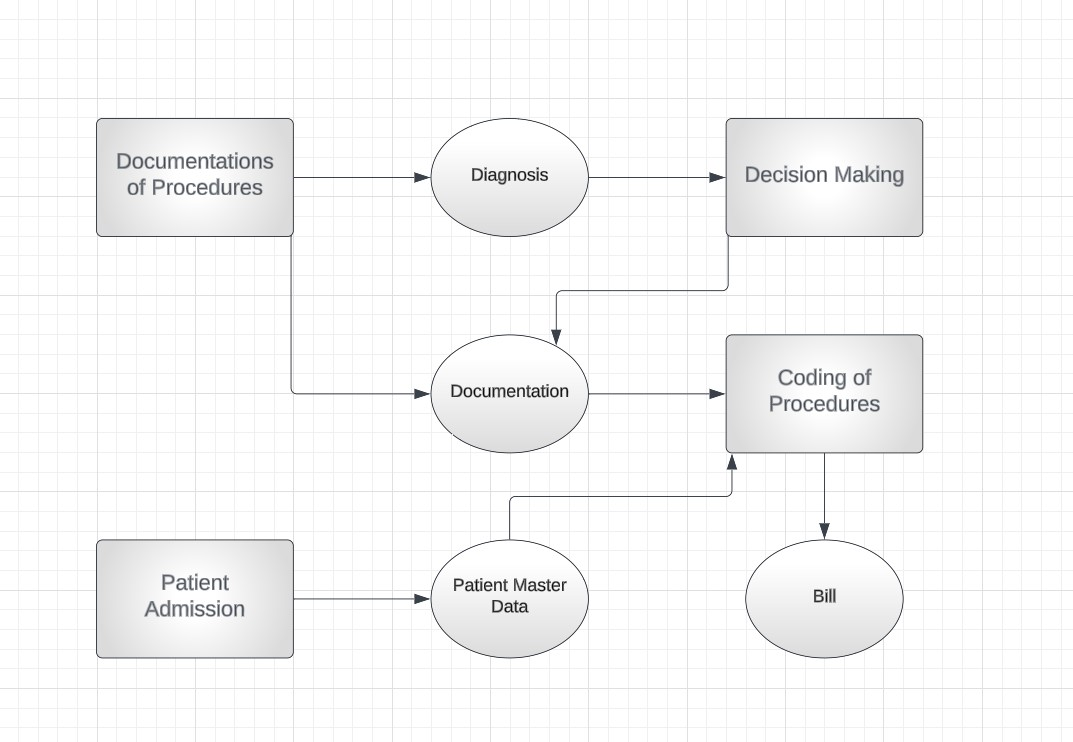
\includegraphics[width=12cm]{src/pic/Typical_Medical_Procedure.jpg}\end{center}
\caption{Typical Medical Structure \cite{Ben20}}
\label{TMP}
\end{figure}


\section{Modeling Concepts}
To effectively design and represent hospital information systems, this paper utilizes modeling concepts such as Monticore and Business Process Model and Notation (BPMN), which are explained a bit further in more detail.

\subsection{Monticore}

Monticore is a domain-specific modeling language and toolset that provides support for modeling, analysis, and code generation. It is widely used in software engineering and system design to create models that capture the structure, behavior, and interactions of complex systems. Monticore facilitates the creation of models using various diagrammatic notations and allows for the specification of model constraints, transformations, and code generation. \cite{Monticore:Framework}

In the context of this paper, Monticore is utilized to create models such as class diagrams, use case diagrams, and sequence diagrams to represent different aspects of hospital information systems. Class diagrams help visualize the structure and relationships between the various entities and data elements within the system. Use case diagrams capture the functionalities and interactions between system users and the system itself. Sequence diagrams illustrate the dynamic behavior and flow of activities within the system, particularly during specific processes or scenarios. 

By utilizing Monticore, this paper leverages a powerful modeling language and toolset to effectively represent and analyze the various components and functionalities of hospital information systems.

Below we will summarize the languages from the Monticore Catalog that we used for modelling various aspects of Hospital Information Systems - 

\subsubsection{Class Diagram For Analysis (CD4A)}
CD4A is a concise textual representation of UML class diagrams, explicitly utilizing the UML/P variant (“P” in UML/P stands for “suitable for programming”). It covers the essential elements of class diagrams, including classes, interfaces, inheritance, attributes with types and visibilities, and various association and composition types, such as qualified and ordered associations. CD4A allows software engineers to represent complex class structures and accurately depict relationships between classes while maintaining code reusability and modularity through inheritance. Including attributes with associated types and visibilities ensures a comprehensive representation of class characteristics. CD4A is a compact, human-readable alternative to graphical UML tools, facilitating collaboration, version control, and documentation.\cite{MontiCore}
 
 
\subsubsection{Sequence Diagrams (SD)}
SD is a textual language that allows for the representation of sequence diagrams (SDs). The project encompasses grammar, a symbol table infrastructure, a PrettyPrinter, and several CoCos for type-checking. The language is divided into two grammars: SDBasis and SD4Development. SDBasis serves as a foundational grammar, providing essential features of the SD language.\cite{MontiCore}


\subsubsection{Use Case Diagrams (UCD)}

UCD is a textual language designed to represent use case diagrams (UCDs). The project comprises a grammar, a symbol table infrastructure, and a semantic differencing operator. The language is defined by the UCD grammar, which provides the necessary syntax and rules to describe use case diagrams.

UCD allows for modelling various elements, including actors, use cases, preconditions, associations between actors and use cases, extend relations between use cases with guards, including relations between use cases, and specialization relations between actors and use cases. These elements capture the interactions and relationships between actors and use cases in a system, visually representing the system's functional requirements.\cite{MontiCore}


\subsection{Business Process Model and Notation (BPMN)}


BPMN is a standardized graphical notation for modeling business processes. It visually represents business workflows, activities, decisions, and the flow of data or information within an organization. BPMN diagrams offer a clear and intuitive way to depict the sequence of activities, decision points, and the involvement of different stakeholders in a process. \footnote{BPMN Website 
\url{https://www.bpmn.org/}.}

In hospital information systems, BPMN diagrams are valuable for modeling and analyzing the workflows and processes involved in patient care, administrative tasks, and other activities within the healthcare organization. BPMN diagrams help stakeholders understand the sequence of activities, identify bottlenecks, and improve the efficiency of processes. 

By utilizing BPMN in this paper, we can effectively represent the complex workflows and interactions within hospital information systems, contributing to a better understanding of the system's behavior and facilitating process optimization. \cite{Aagesen2015}



\begin{figure}[!htb]
\begin{center}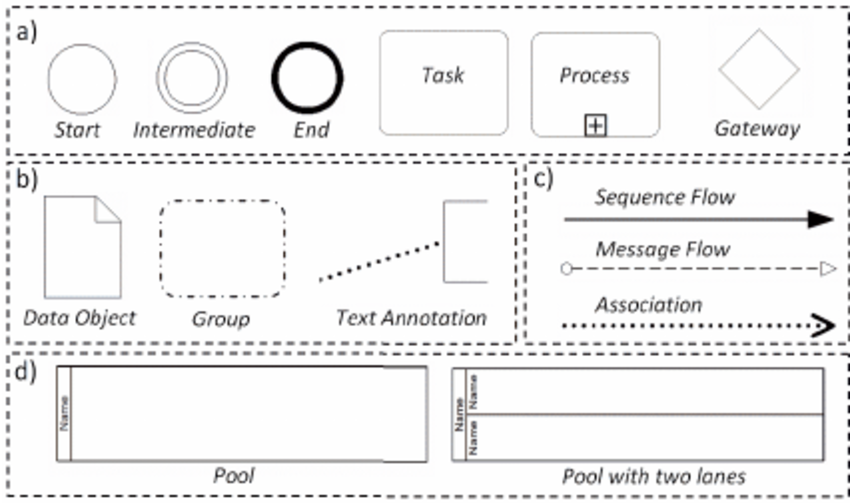
\includegraphics[width=12cm]{src/pic/Basic_BPMN.png}\end{center}
\caption{Basic Elements of BPMN 2.0 \cite{BPMN_Basic}}
\label{BBPMN}
\end{figure}


\let\cleardoublepage\clearpage

\chapter{Models and Documentation}\label{ch:listings}
%% use language 'myLng' for the next listings (until another language is set)
%% include listing 'listings/AdverseReactionApp.aj' with label and caption
%% note: big listings sometimes need to overwrite the float value that has been
%% already set in the general listings setup (see paper.tex)

% This chapter contains the beautiful listing \ref{lst:system}. 

In this section, we present the models developed for the hospital information system using Monticore, a domain-specific modeling language and toolset, as well as Business Process Model and Notation (BPMN) diagrams. The models serve as visual representations of the system's structure, behavior, and interactions, offering stakeholders a comprehensive understanding of the various components and functionalities of the hospital information system.

\section{Class Diagrams}

% \begin{landscape}
\begin{figure}[htbp]
  \centering
  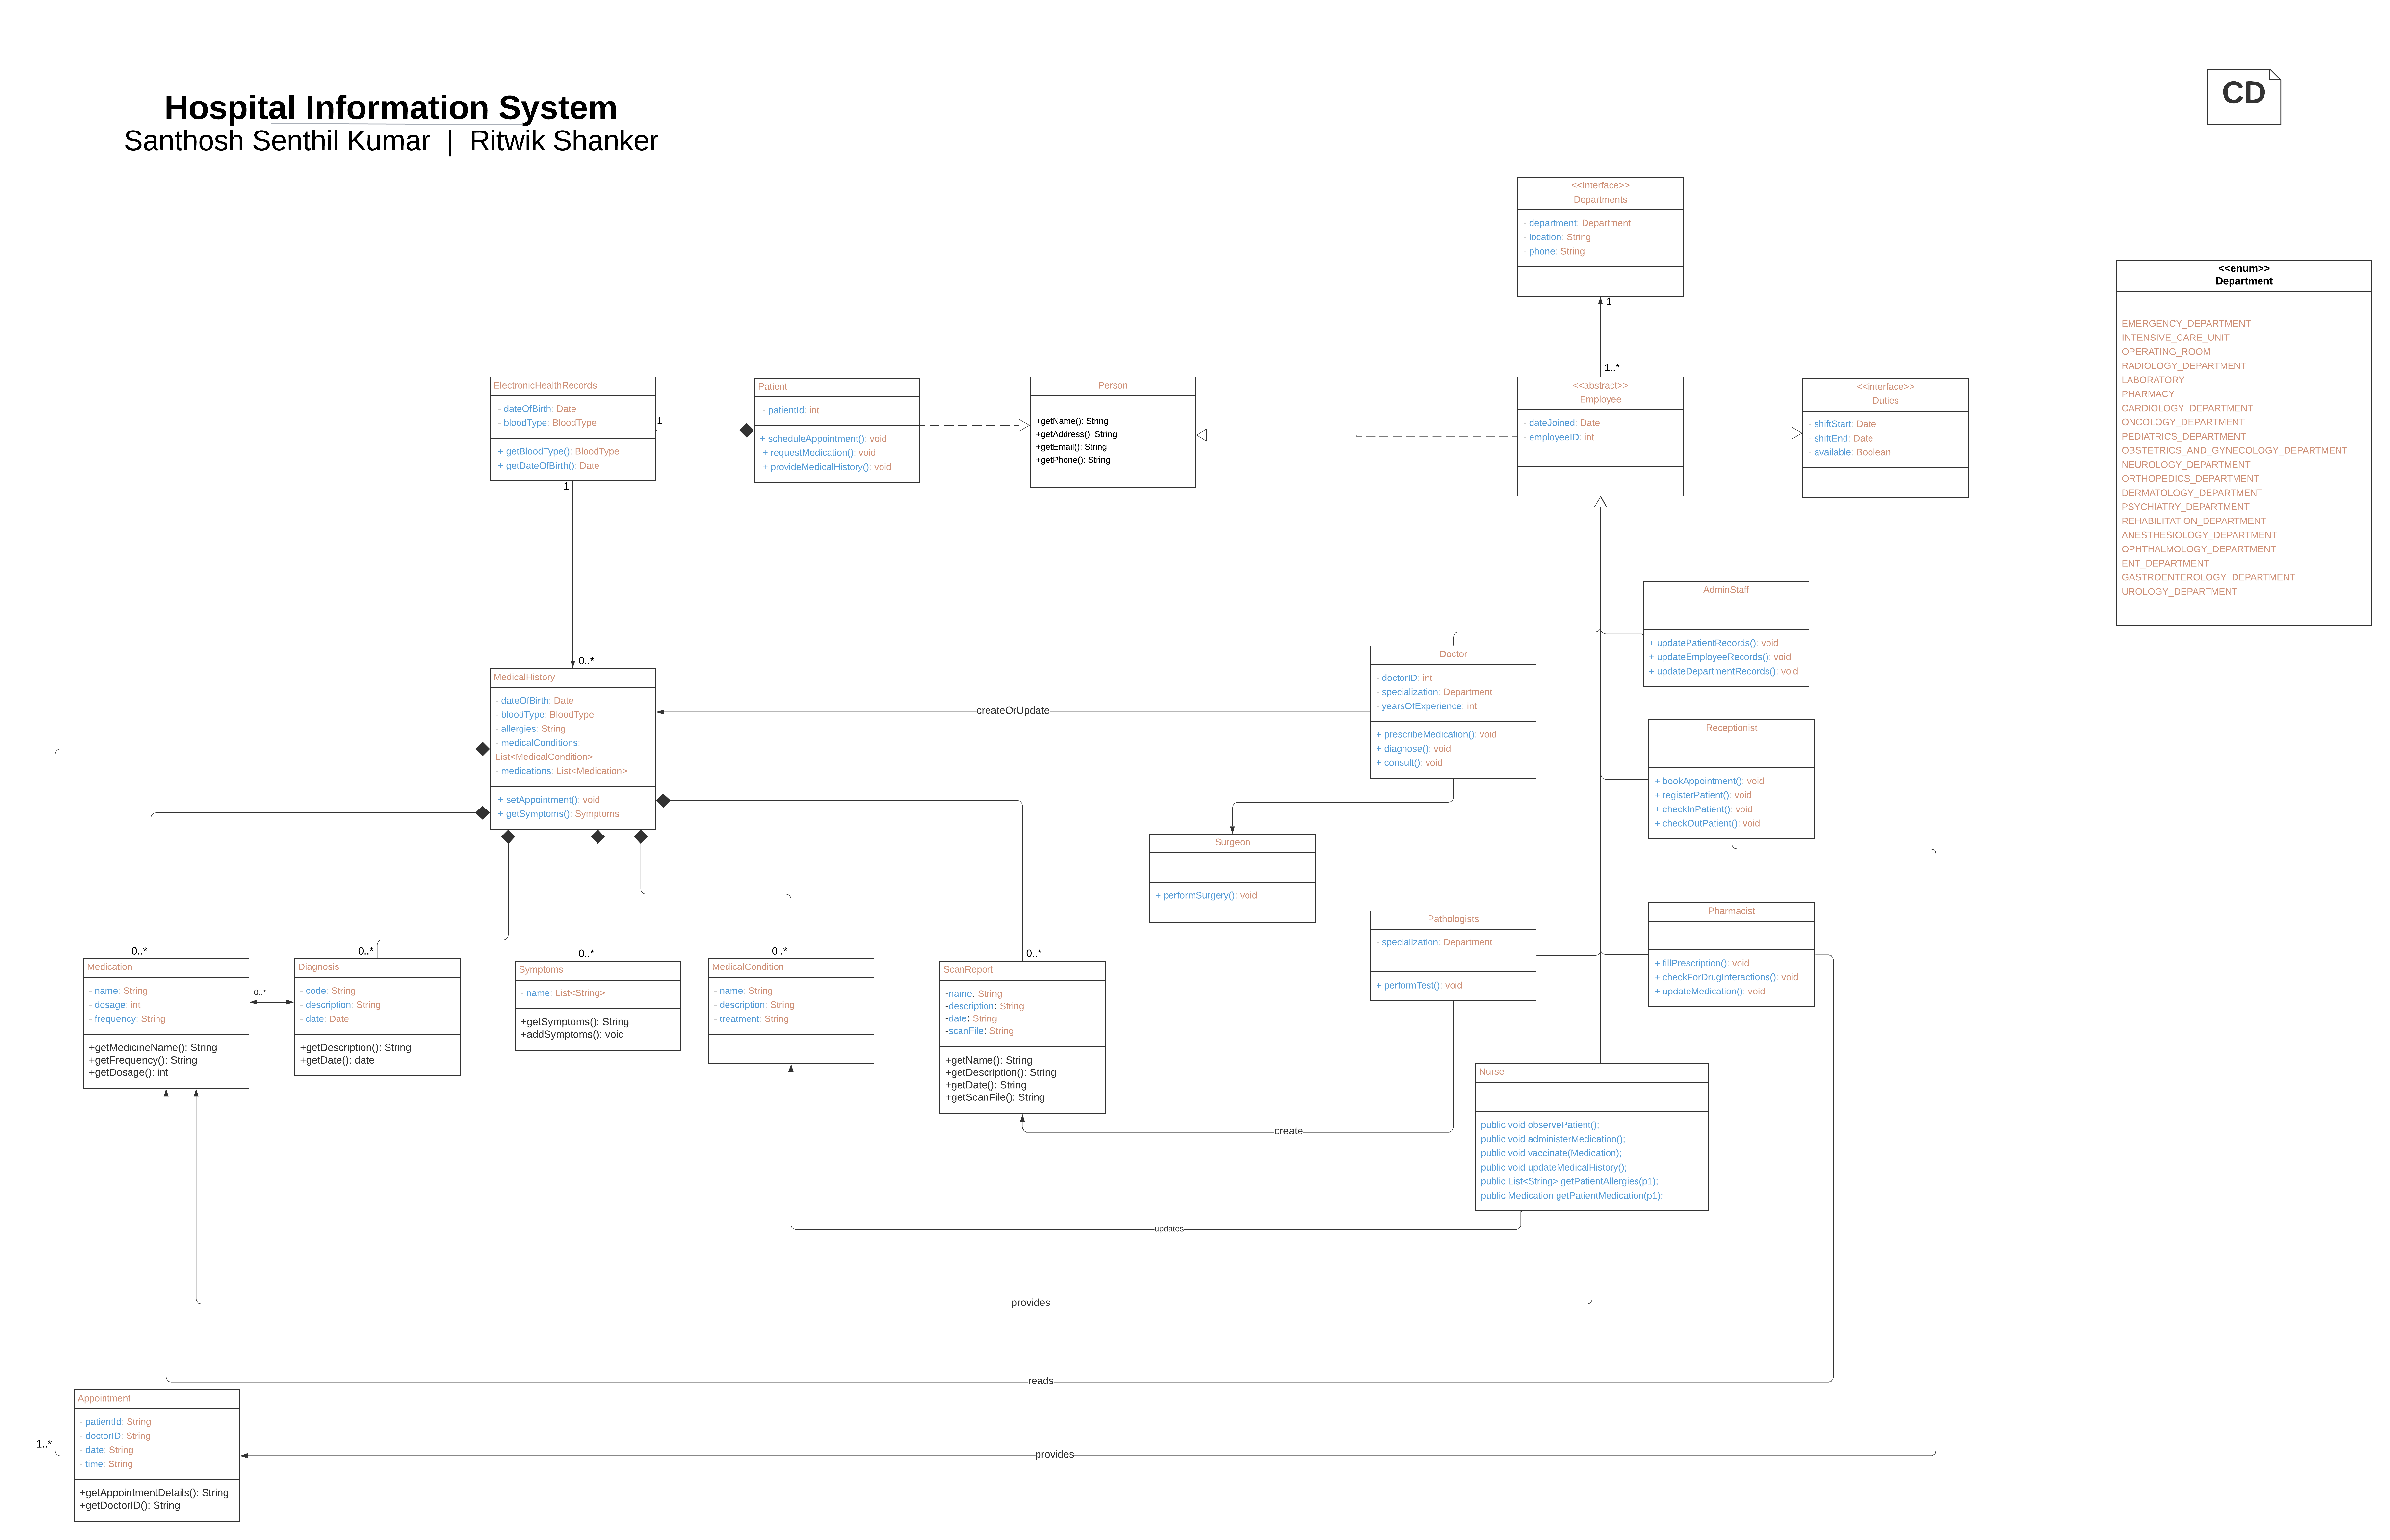
\includegraphics[width=\textwidth,height=\textheight,keepaspectratio]{src/pic/UML class.png}
  \caption{Visual Representation of Class Diagram showing all the classes}
  \label{fig:fullscreen}
\end{figure}
% \end{landscape}



\subsection{Patient}
\begin{figure}[hbt]
\lstset{language=MontiArc}
\lstinputlisting[
label=lst:patientcd,
caption=Class Diagram for Patient Class] {src/listings/CD/Patient.cd}
\end{figure}

The \texttt{Patient} class represents a patient in a healthcare system. It extends the \texttt{Person} class and adds additional attributes specific to patients. The \texttt{Person} class contains common attributes such as ID, name, address, email, and phone.

The \texttt{Patient} class has the following operations:
\begin{itemize}
  \item \texttt{scheduleAppointment()}: Allows the patient to schedule an appointment.
  \item \texttt{requestMedication()}: Allows the patient to request medication.
  \item \texttt{provideMedicalHistory()}: Allows the patient to provide their medical history.
\end{itemize}

The \texttt{Patient} class has a composition relationship with the \texttt{MedicalHistory} class, indicating that each patient has a medical history. This relationship is denoted by the arrow connecting \texttt{Patient} to \texttt{MedicalHistory} with a multiplicity of \texttt{[*]}, meaning each patient can have multiple medical history records.

\subsection{Hospital}
\lstinputlisting[language=MontiArc,breaklines=true,caption=Class Diagram for Hospital Class]{src/listings/CD/Hospital.cd}

% \begin{figure}[hbt]
% \lstset{language=MontiArc}
% \lstinputlisting[
% label=lst:hospcd,
% caption=Class Diagram for Hospital Class] {src/listings/CD/Hospital.cd}
% \end{figure}

The \texttt{Hospital} class has the following nested classes:
\begin{itemize}
  \item \texttt{Departments}: Represents a department in the hospital. It has attributes such as the department name, location, and phone number.
  \item \texttt{Receptionist}, \texttt{Nurse}, \texttt{Pharmacist}, \texttt{AdminStaff}, \texttt{Pathologists}, \texttt{Doctor}, and \texttt{Surgeon}: These classes represent different types of employees in the hospital. They extend the \texttt{Employee} class, which itself extends the \texttt{Person} class. Each employee class has specific operations related to their role in the hospital.
\end{itemize}


The \texttt{Hospital} class also has an enumeration called \texttt{Department}, which lists various departments in the hospital.

There are associations between the classes:
\begin{itemize}
  \item \texttt{Employee} has a composition relationship with \texttt{Duties}, indicating that each employee has one or more duties.
  \item \texttt{AdminStaff} has a supervision relationship with other employees, denoted by the association between \texttt{AdminStaff} and \texttt{Employee}.
  \item \texttt{Doctor} has a relationship with \texttt{Departments}, indicating that each doctor can head a department, and each department can have a head doctor.
  \item \texttt{Employee} has a relationship with \texttt{Departments}, indicating that each employee works in one department.
\end{itemize}

\subsection{Electronic Health Record}

\lstinputlisting[language=MontiArc,breaklines=true,caption=Class Diagram for EHR Class]{src/listings/CD/EHR.cd}
% \begin{figure}[hbt]
% \lstset{language=MontiArc}
% \lstinputlisting[
% label=lst:ehrcd,
% caption=Class Diagram for EHR Class] {src/listings/CD/EHR.cd}
% \end{figure}

The \texttt{EHR} class represents an Electronic Health Record (EHR) system. It contains several classes related to medical information.

The \texttt{EHR} class has the following nested classes:
\begin{itemize}
  \item \texttt{Symptoms}: Represents a list of symptoms.
  \item \texttt{Diagnosis}: Represents a medical diagnosis with attributes such as code, description, date, and associated symptoms.
  \item \texttt{ScanReport}: Represents a scan report with attributes such as name, description, date, and the file containing the scan.
  \item \texttt{Appointment}: Represents a scheduled appointment with attributes such as patient ID, doctor ID, date, and time.


  \item \texttt{Medication}: Represents a medication with attributes such as name, dosage, and frequency.
  \item \texttt{MedicalCondition}: Represents a medical condition with attributes such as name, description, and treatment. The treatment attribute within the MedicalCondition class allows for the inclusion of information related to the recommended or prescribed procedures, medications, therapies, or lifestyle modifications that are commonly associated with managing or treating that specific medical condition.
\end{itemize}

The \texttt{MedicalHistory} class is an abstract class representing the medical history of a patient. It contains attributes and relationships to various medical components such as allergies, medical conditions, medications, diagnoses, symptoms, scan reports, and appointments.

There are composition relationships between \texttt{MedicalHistory} and each of the medical components, indicating that a medical history consists of multiple instances of these components.

The \texttt{ElectronicHealthRecord} class represents an electronic health record for a patient. It contains attributes such as date of birth and blood type. It has a composition relationship with \texttt{MedicalHistory}, indicating that an electronic health record includes a patient's medical history.


\section{Sequence Diagrams}


\subsection{Patient Scan}

\begin{figure}[]
\lstset{language=MontiArc}
\lstinputlisting[
label=lst:pssd,
caption=Sequence Diagram for patient getting scanned] {src/listings/SD/patient-scan.sd}
\end{figure}

\begin{figure}[htb]
\begin{center}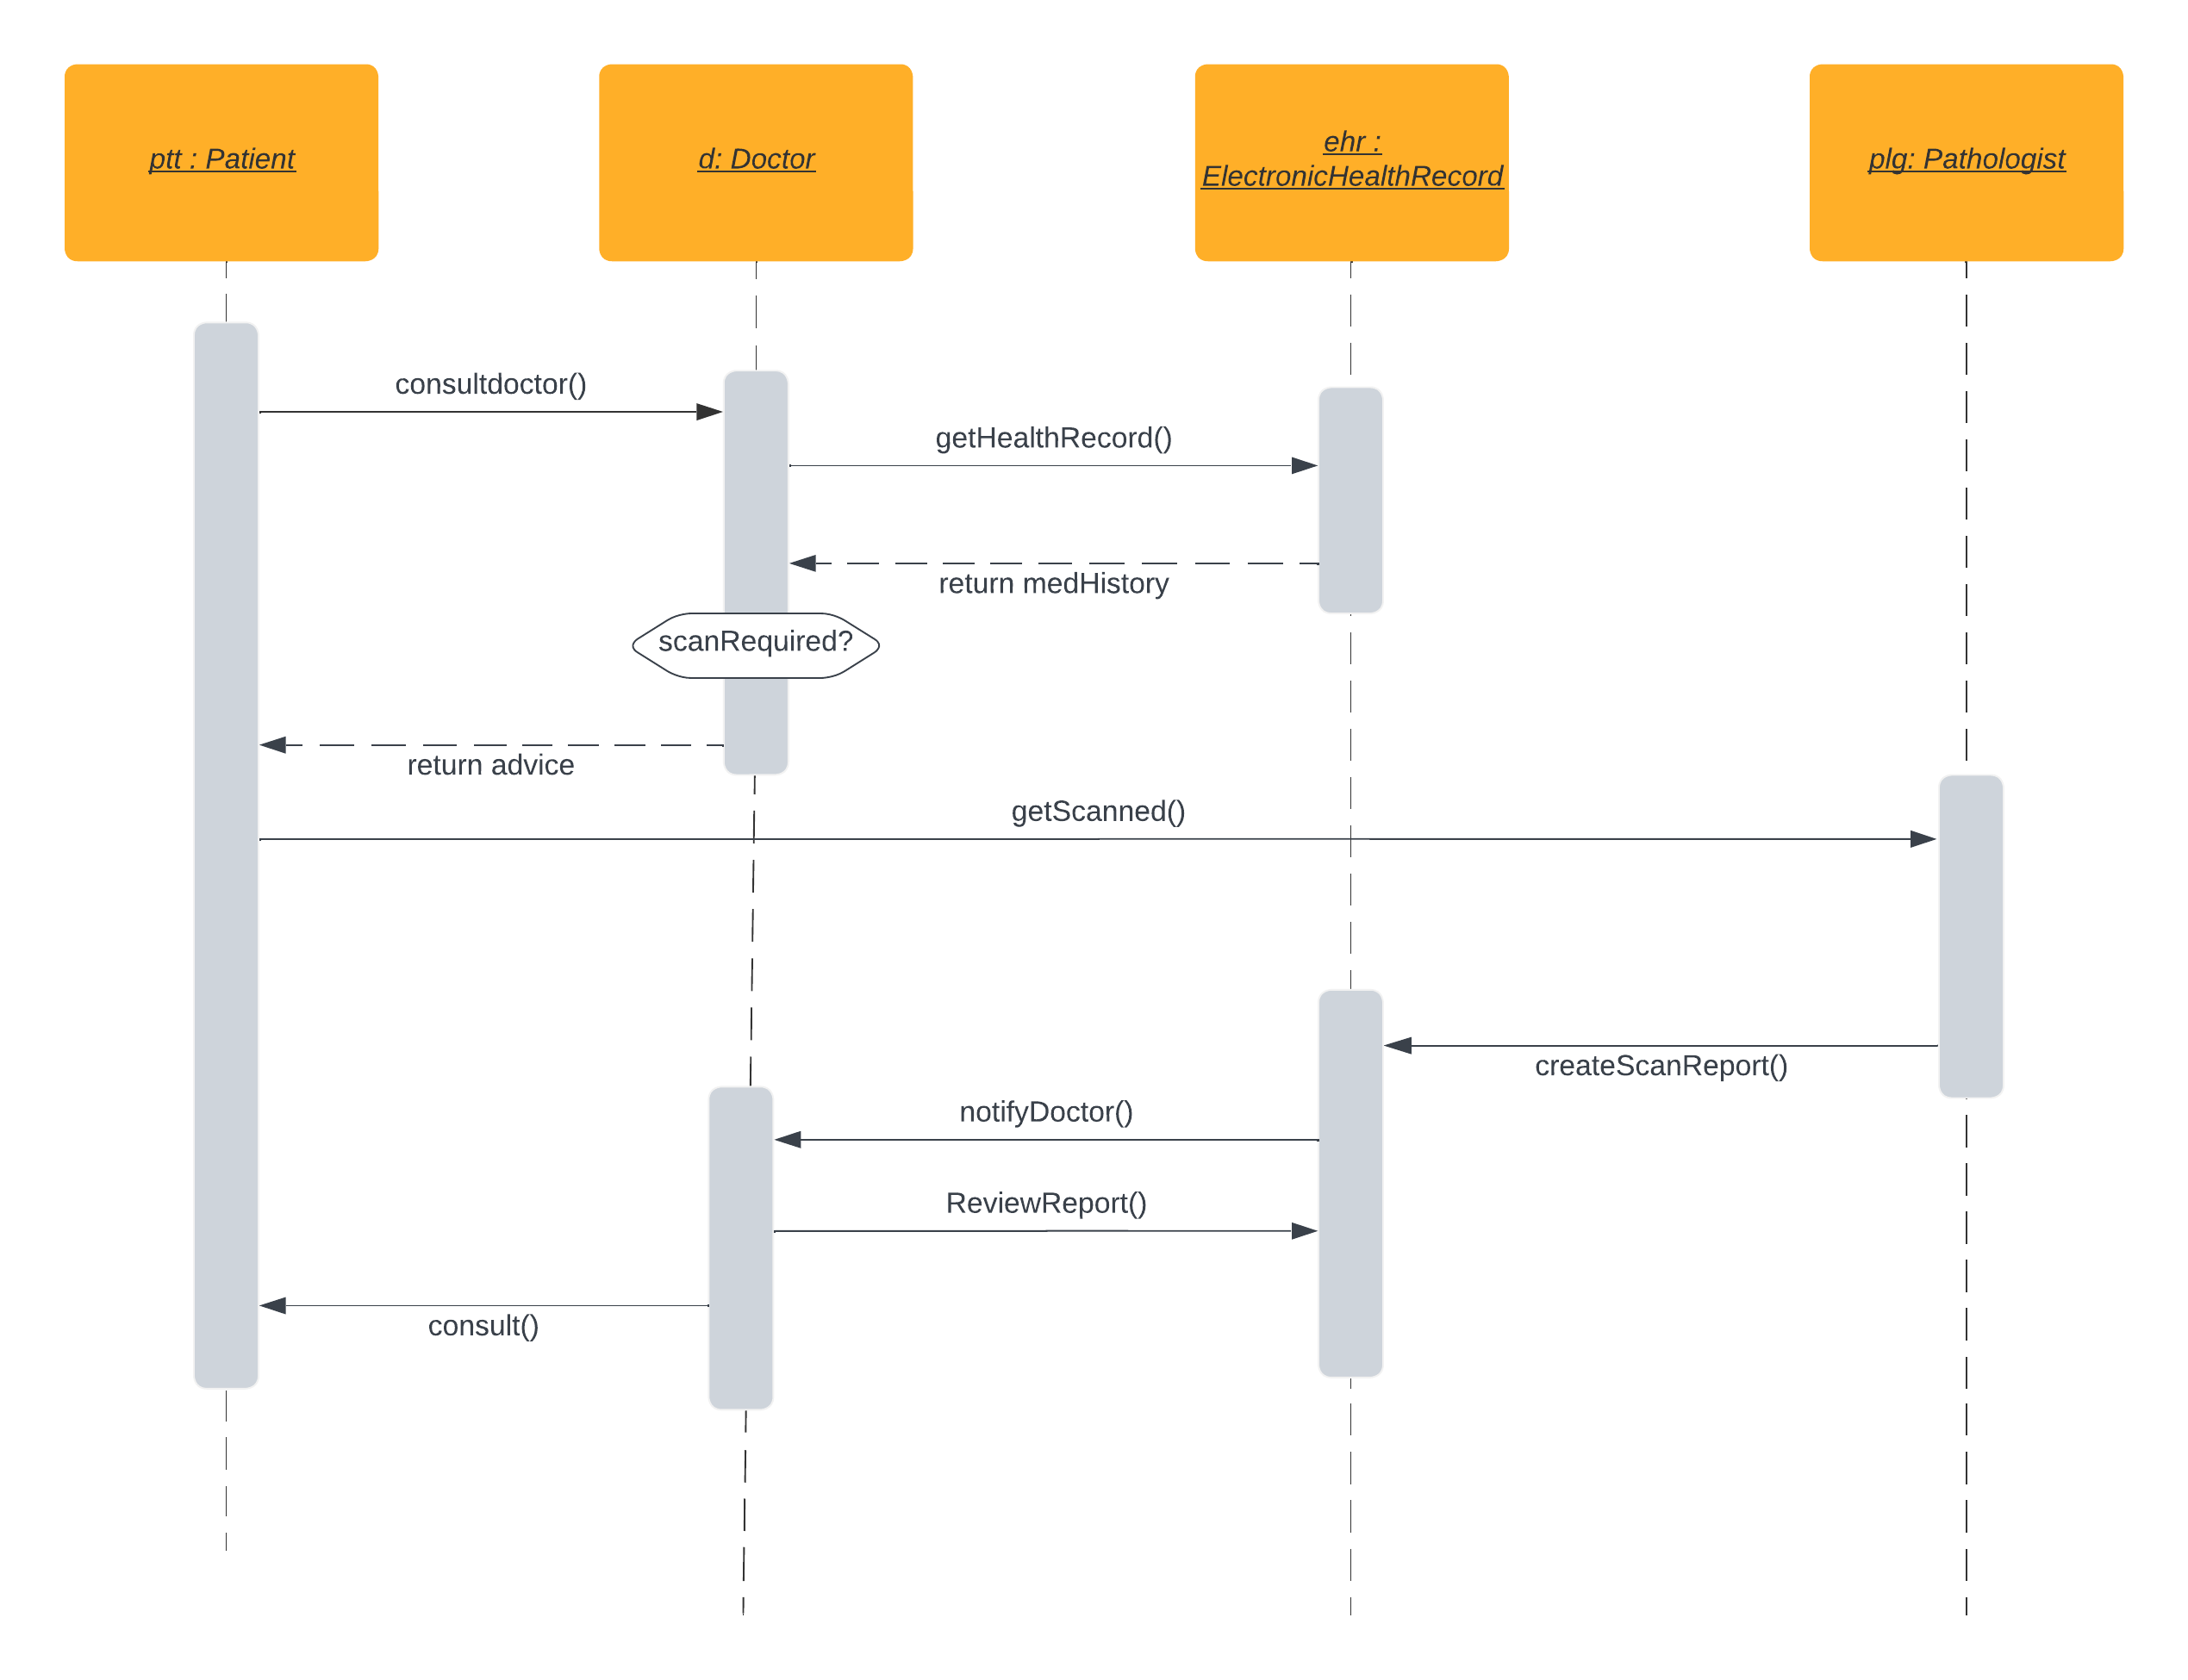
\includegraphics[width=12cm]{src/pic/SD1.png}\end{center}
\caption{Visual Sequence Diagram for Patient Scan process}
\label{SD1}
\end{figure}

The sequence diagram illustrates the interaction between a patient (\texttt{pt}), a doctor (\texttt{d}), an electronic health record (\texttt{ehr}), and a pathologist (\texttt{plg}) during a scanning process.

\begin{enumerate}
\item The patient initiates the \texttt{consultdoctor()} operation with the doctor.
\item The doctor retrieves the patient's health record from the electronic health record (\texttt{ehr}) using the \texttt{getHealthRecord(pt)} operation.
\item The electronic health record returns the medical history (\texttt{medHistory}) to the doctor.
\item The doctor verifies if a scan is required by checking the \texttt{scanRequired} attribute of the medical history. If it is true, the process continues; otherwise, the doctor provides advice to the patient and the sequence ends.
\item The doctor informs the patient of their advice using the \texttt{return advice} operation.
\item The patient requests the pathologist (\texttt{plg}) to get scanned by invoking the \texttt{getScanned()} operation.
\item The pathologist creates a scan report (\texttt{scanReport}) and sends it to the electronic health record using the \texttt{createScanReport(scanReport)} operation.
\item The electronic health record receives the scan report and acknowledges the pathologist.
\item The electronic health record notifies the doctor about the scan report using the \texttt{notifyDoctor(scanReport)} operation.
\item The doctor reviews the scan report using the \texttt{reviewReport()} operation.
\item The doctor consults with the patient using the \texttt{consult()} operation.
\item The patient responds to the doctor's consultation.
\item The doctor updates the medical history in the electronic health record using the \texttt{addHistory()} operation.
\end{enumerate}

\subsection{Vaccination}

The sequence diagram depicts the interaction between a patient (\texttt{p1}), a nurse (\texttt{nu1}), and an electronic health record (\texttt{ehr}) during a vaccination process that involves checking for allergies and using anti allergant along with the vaccine. This has been broken down into two parts, one for patient without allergies and one for with allergies.


\subsubsection{Vaccination of patient without allergies}
% \lstinputlisting[language=MontiArc,breaklines=true,caption=Class Diagram for EHR Class]{src/listings/CD/EHR.cd}




The sequence of events is as follows:

\begin{enumerate}
\item The patient arrives at the hospital and initiates the \texttt{arriveToHospital()} operation with the nurse.
\item The nurse retrieves the patient's allergies from the electronic health record using the \texttt{getAllergies(p1)} operation.
\item The electronic health record returns no allergies to the nurse.
\item The nurse administers the vaccination to the patient.
\item The nurse observes the patient and initiates the \texttt{ObservePatient()} operation.
\item The nurse updates the patient's medical history in the electronic health record using the \texttt{UpdateMedicalHistory()} operation.
\item The patient responds to the nurse's observation.
\end{enumerate}

\lstinputlisting[
label=lst:vpsd,
language=MontiArc,breaklines=true,
caption=Sequence Diagram for patient getting vaccinated without allergies] {src/listings/SD/vaccination.sd}

\begin{figure}[]
\begin{center}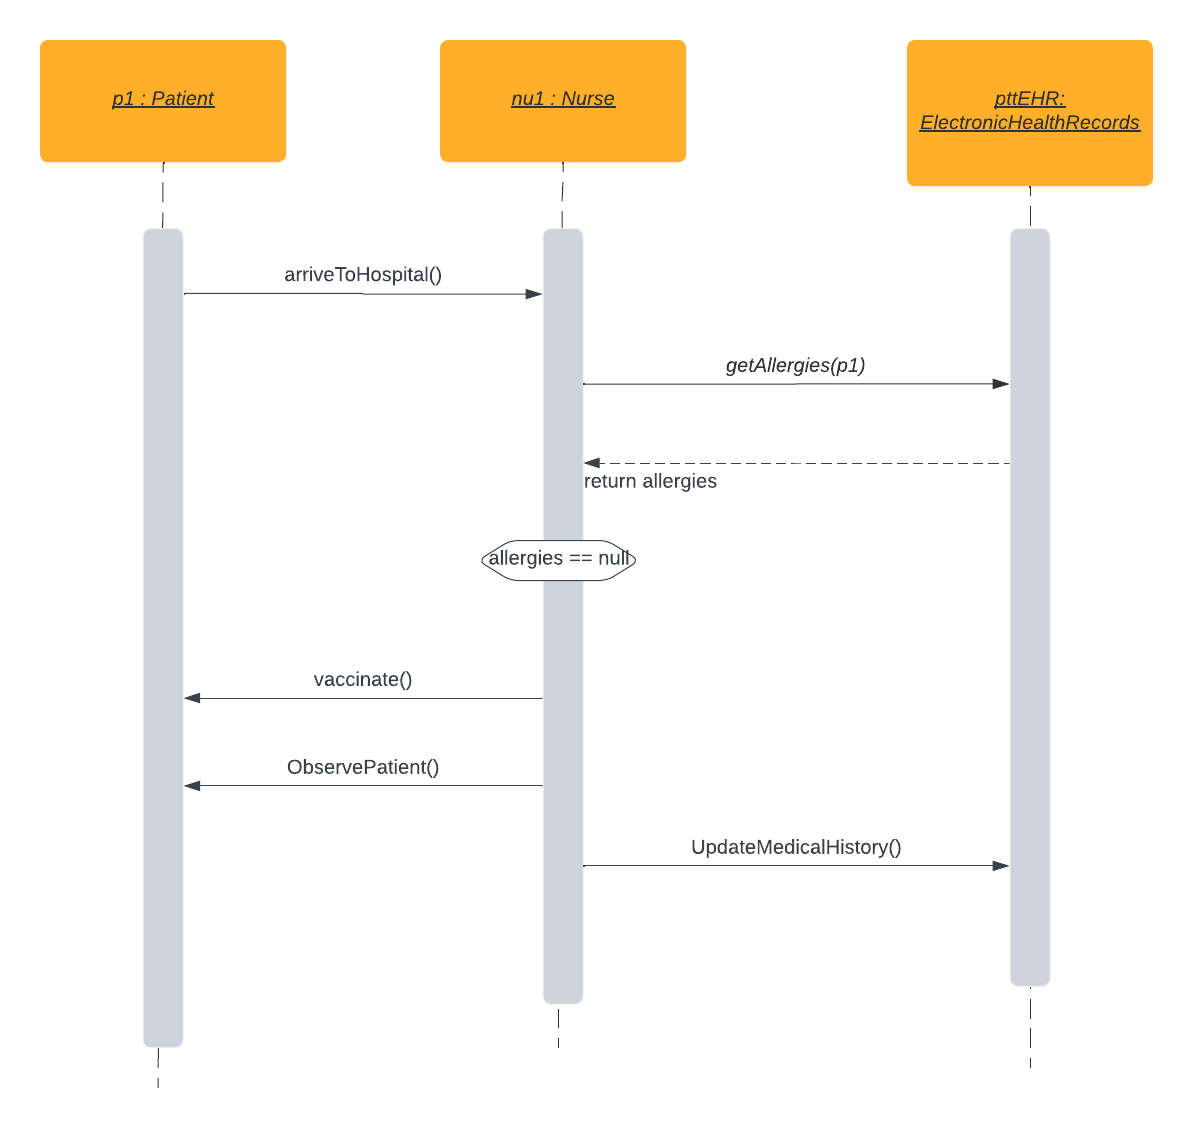
\includegraphics[width=12cm, height = 9cm]{src/pic/Vaccination_Without_Allergies.png}\end{center}
\caption{Visual Sequence Diagram for Vaccination of a Patient without Allergies}
\label{VAC1}
\end{figure}

\subsubsection{Vaccination of patient with allergies}

\begin{figure}[hbt]
\lstset{language=MontiArc}
\lstinputlisting[
label=lst:vpasd,
caption=Sequence Diagram for patient getting vaccinated without allergies] {src/listings/SD/vaccination-allergies.sd}
\end{figure}

\begin{enumerate}
\item The patient arrives at the hospital and initiates the \texttt{arriveToHospital()} operation with the nurse.
\item The nurse retrieves the patient's allergies from the electronic health record using the \texttt{getAllergies(p1)} operation.
\item The electronic health record returns the allergies to the nurse.
\item The nurse retrieves the patient's medication history (\texttt{mc1}) from the electronic health record using the \texttt{getMedication(p1)} operation.
\item The electronic health record returns the medication history to the nurse.
\item The nurse checks for an anti-allergen (\texttt{antiAllergent}) based on the medication history.
\item The nurse administers the vaccination to the patient, taking into account the anti-allergen.
\item The nurse observes the patient and initiates the \texttt{ObservePatient()} operation.
\item The nurse updates the patient's medical history in the electronic health record using the \texttt{UpdateMedicalHistory()} operation.
\item The patient responds to the nurse's observation.
\end{enumerate}

\begin{figure}[htb]
\begin{center}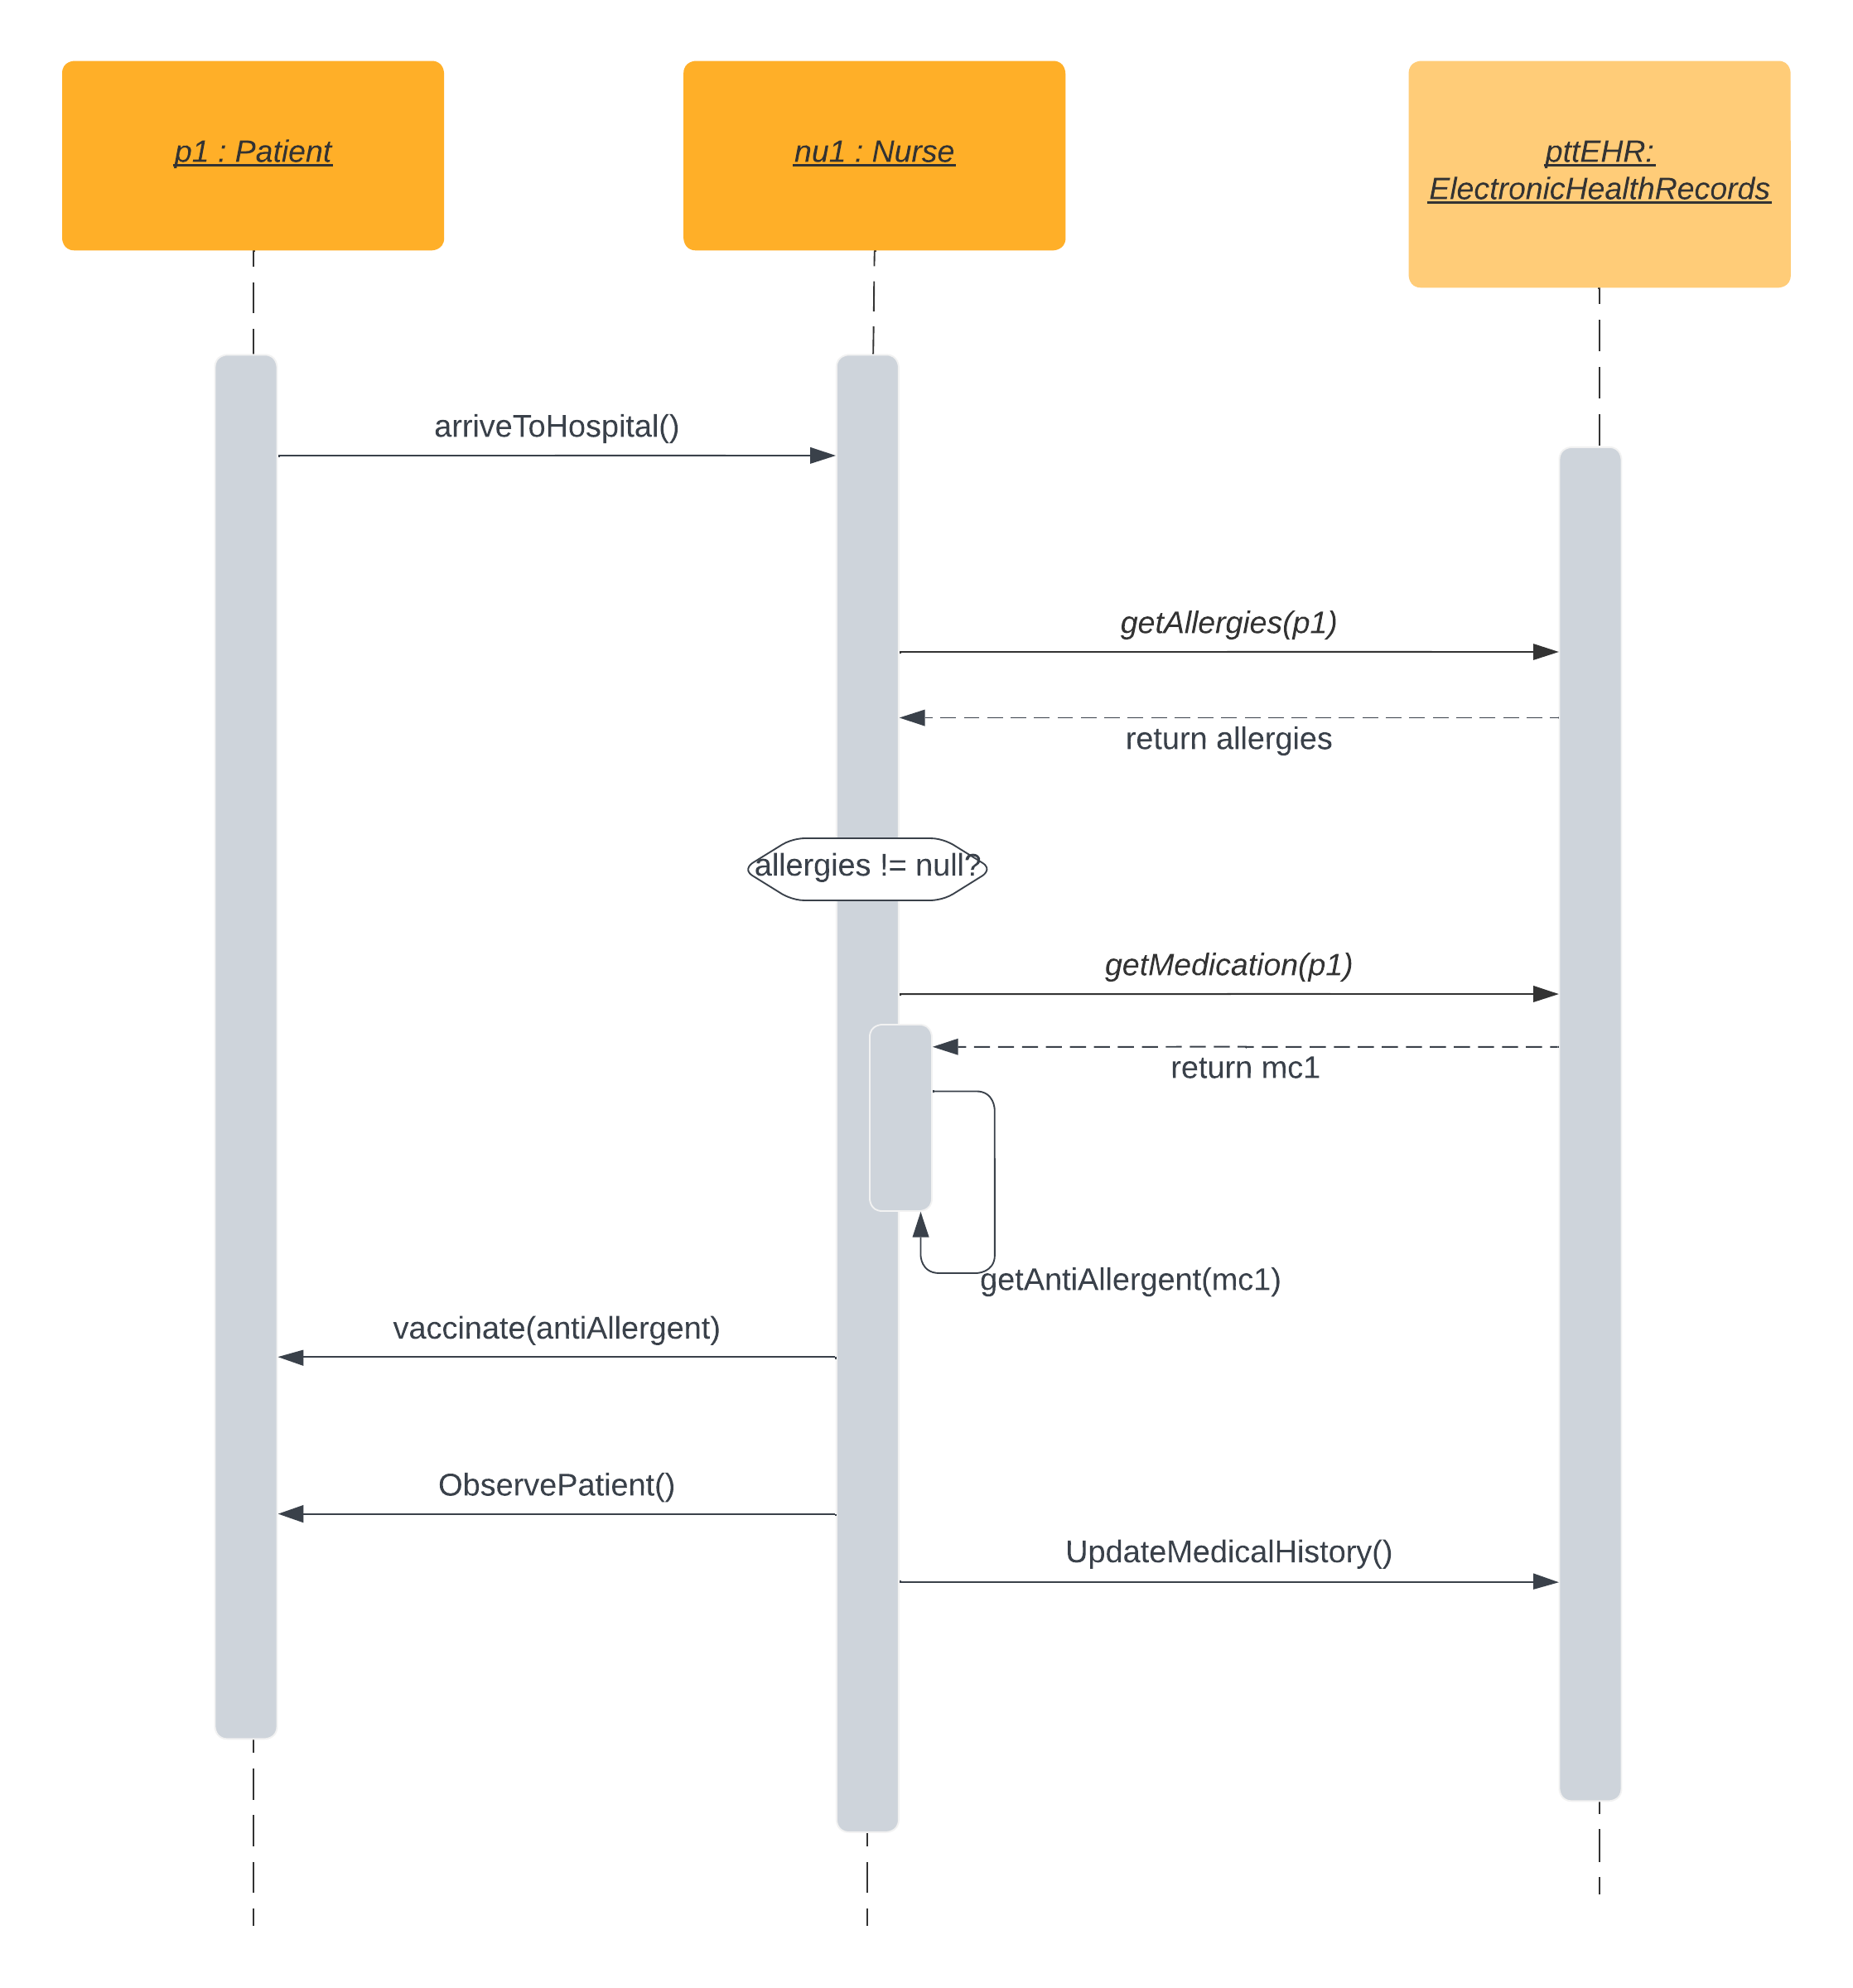
\includegraphics[width=12cm]{src/pic/Vaccination_With_allergies.png}\end{center}
\caption{Visual Sequence Diagram for Vaccination of a Patient with Allergies}
\label{VACA2}
\end{figure}


\section{Use Case Diagram}

\subsection{Reception and Patient UCD}
This use case diagram illustrates the various interactions and functionalities between a receptionist and a patient in the hospital information system.

\textbf{Use Cases}
\begin{itemize}
    \item ScheduleAppointment: This use case allows the receptionist and the patient to schedule an appointment for a specific date and time.
    \item ScheduleHospitalAdmission: The receptionist and the patient can use this use case to schedule a hospital admission for the patient.
    \item PatientRegistration: This use case enables the receptionist and the patient to complete the patient registration process.
    \item PatientHospitalAdmission: The receptionist can initiate the patient's hospital admission process using this use case.
    \item FileMedicalReports: The receptionist can use this use case to file and manage the patient's medical reports.
\end{itemize}

\textbf{Actors}
\begin{itemize}
    \item Receptionist: Represents the hospital receptionist who interacts with the patient and performs administrative tasks.
    \item Patient: Represents the individual seeking medical care from the hospital.
\end{itemize}

\textbf{Relationships}
\begin{itemize}
    \item The Receptionist actor is associated with several use cases, including ScheduleAppointment, ScheduleHospitalAdmission, PatientRegistration, PatientHospitalAdmission, and FileMedicalReports.
    \item The Patient actor is associated with ScheduleAppointment, ScheduleHospitalAdmission, and PatientRegistration.
    \item PatientRegistration extends both ScheduleHospitalAdmission and ScheduleAppointment, indicating that patient registration involves scheduling hospital admissions and appointments.
    \item PatientHospitalAdmission includes PatientRegistration, indicating that the patient's hospital admission process includes patient registration.
    \item NewPatientHospitalAdmission specializes PatientHospitalAdmission, indicating a specific type of patient hospital admission for new patients.
    \item InHospitalPatientAdmission specializes PatientHospitalAdmission, representing the hospital admission process for existing inpatients.
    \item Both NewPatientHospitalAdmission and InHospitalPatientAdmission include BedAllotment, indicating that bed allotment is part of the respective admission processes.
\end{itemize}

\begin{figure}[!htb]
\lstset{language=MontiArc}
\lstinputlisting[
label=lst:recpat,
caption=Use Case Diagram in Moticore UCD] {src/listings/UCD/receptionist_patient.ucd}
\end{figure}


\begin{figure}[!htb]
\begin{center}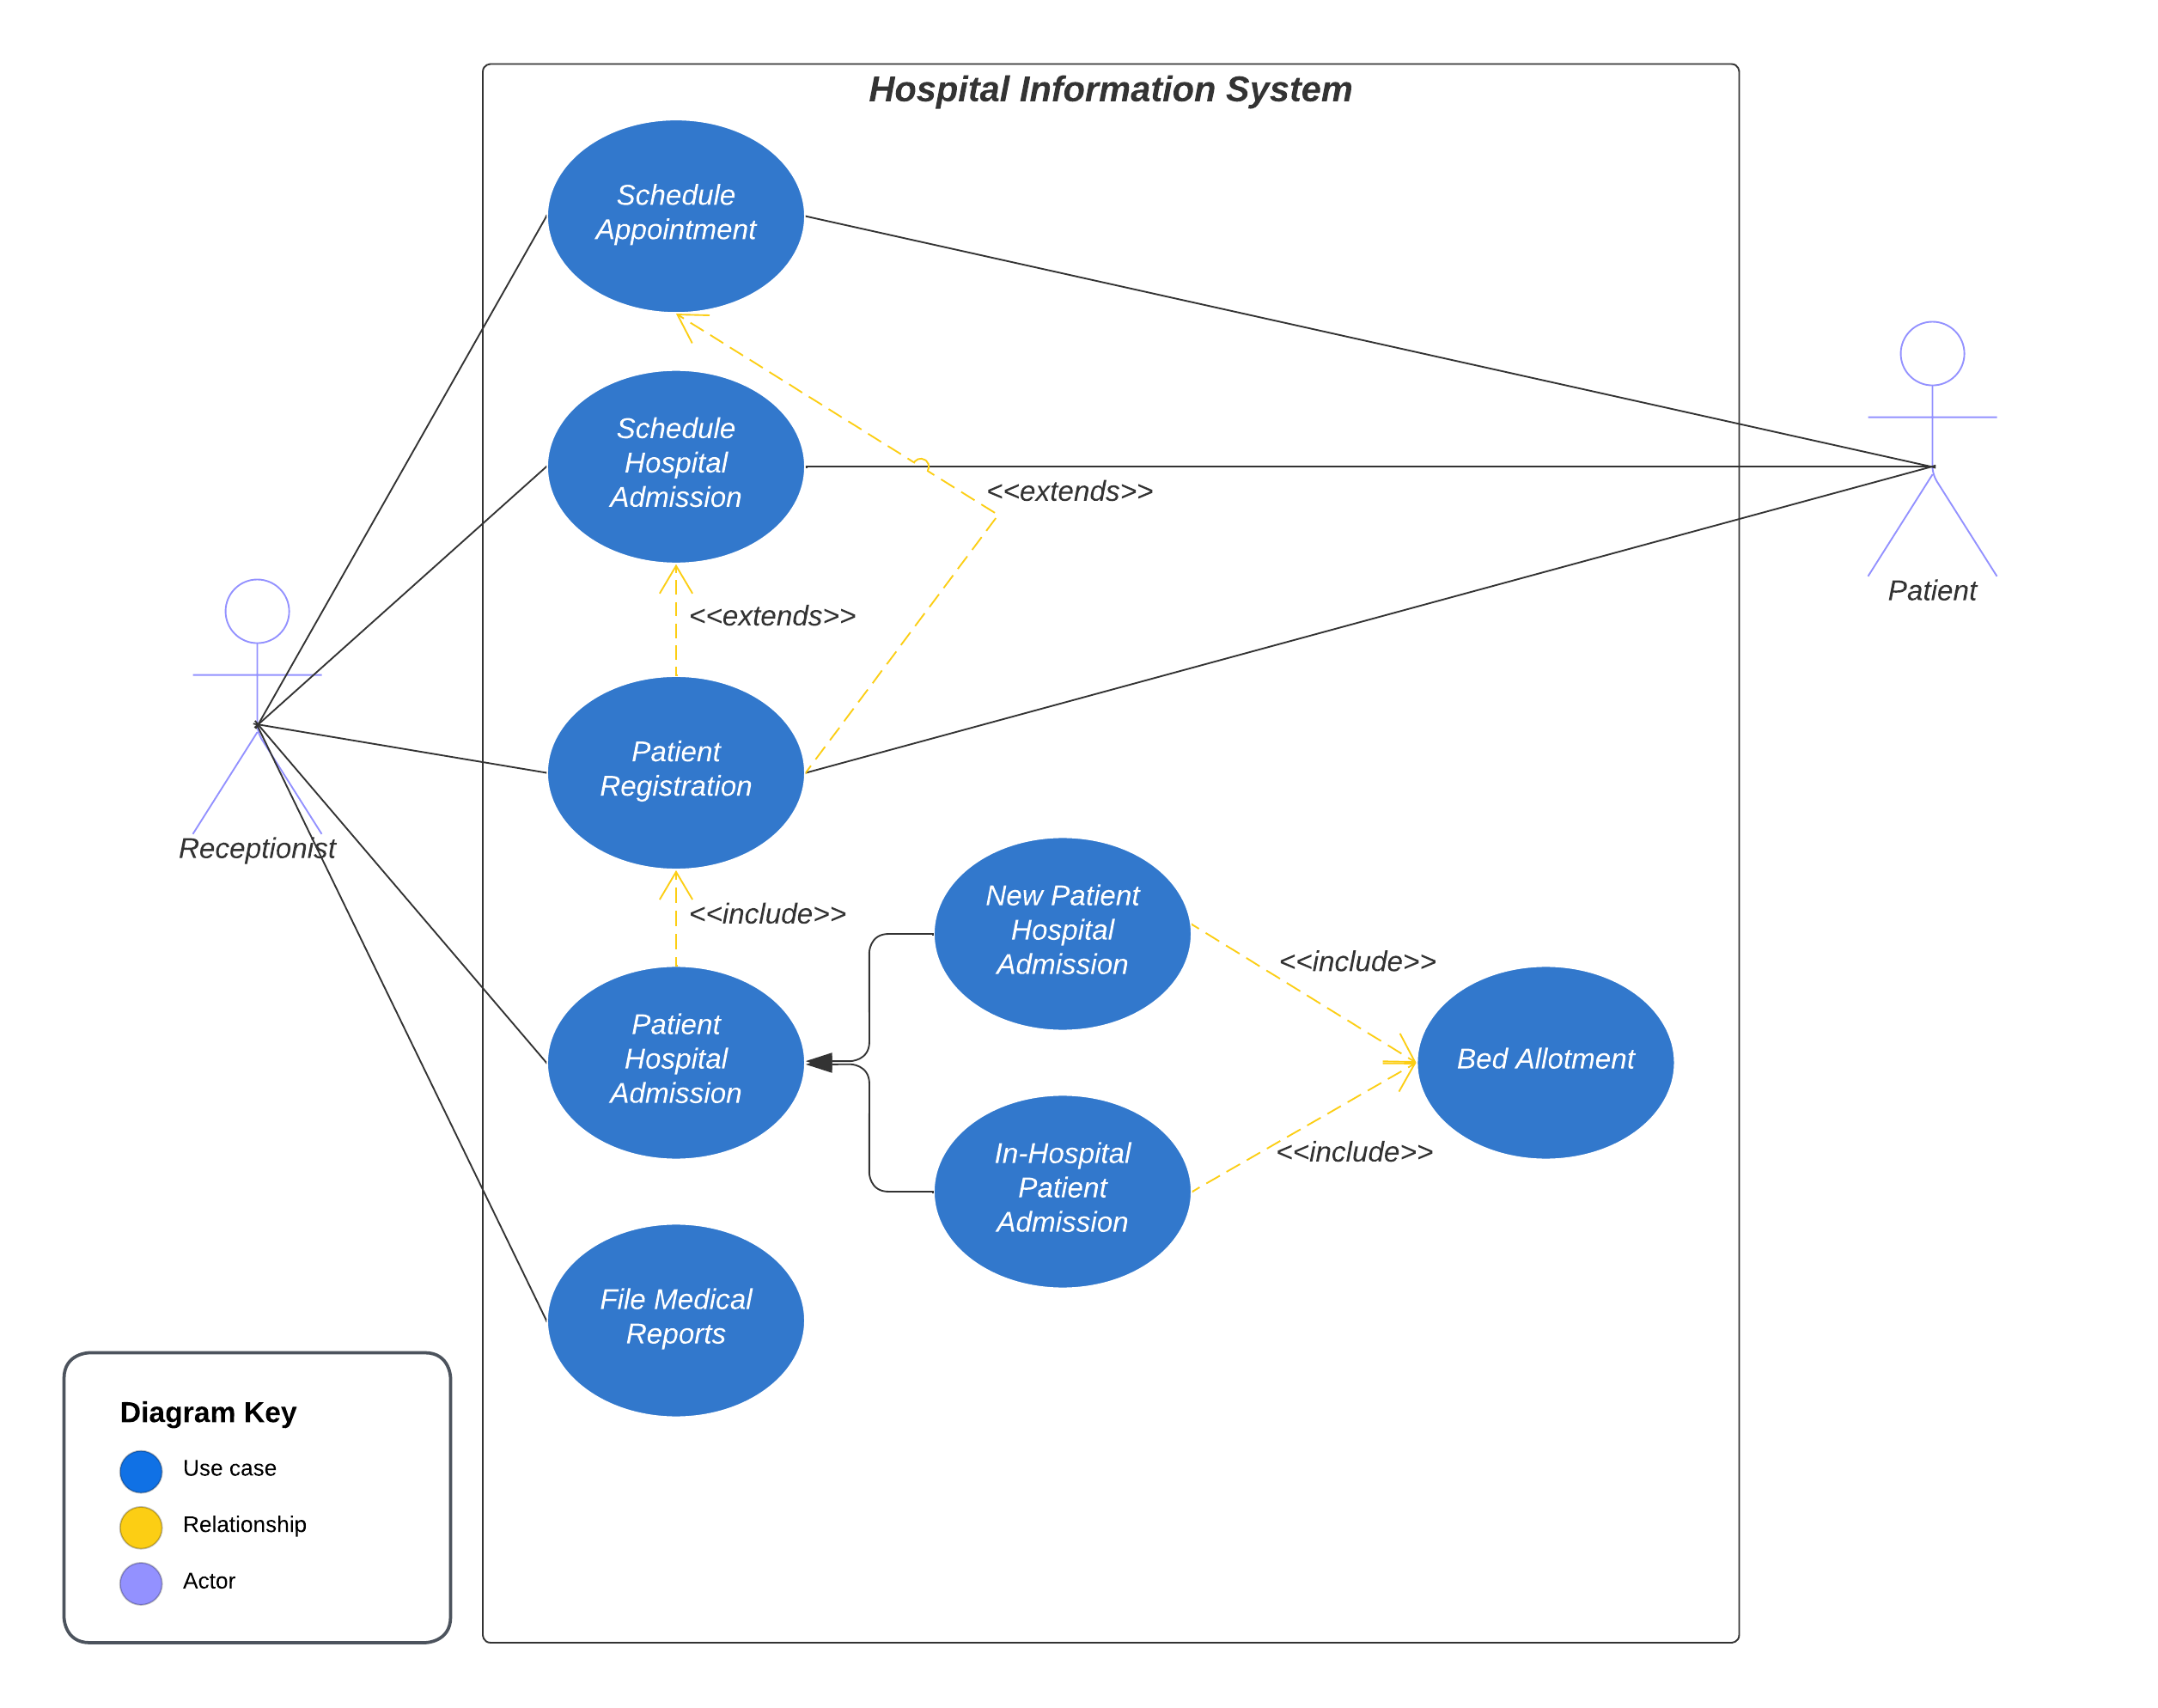
\includegraphics[width=12cm]{src/pic/Diagrams/Receptionist_Patient_UCD.png}\end{center}
\caption{Visual Use Case Diagram of Reception and Patient Case}
\label{RPUCD}
\end{figure}

\subsection{Dischage Patient UCD}

This use case diagram illustrates the interactions and functionalities related to the discharge of a patient from a hospital in the hospital information system.

\textbf{Use Cases}
\begin{itemize}
    \item DischargePatient: Represents the use case where the receptionist performs the patient discharge process.
    \item GenerateBill: This use case extends the ViewEHRs use case and involves generating the patient's bill as part of the discharge process.
\end{itemize}

\textbf{Actors}
\begin{itemize}
    \item Receptionist: Represents the hospital receptionist who is responsible for initiating and managing the discharge process.
\end{itemize}

\textbf{Relationships}
\begin{itemize}
    \item The Receptionist actor is associated with the DischargePatient use case, indicating that the receptionist is responsible for performing the patient discharge process.
    \item GenerateBill extends the ViewEHRs use case, indicating that generating the patient's bill is an additional step within the discharge process.
    \item DischargePatient includes the GenerateBill use case, indicating that generating the bill is a part of the overall discharge process.
    \item DischargeOutPatient specializes the DischargePatient use case, representing the discharge process for patients who were treated as outpatients.
    \item DischargeInPatient specializes the DischargePatient use case, representing the discharge process for patients who were admitted to the hospital as inpatients.
\end{itemize}


\begin{figure}[!htb]
\lstset{language=MontiArc}
\lstinputlisting[
label=lst:dispat,
caption=Use Case Diagram in Moticore UCD for Discharge Patient Use Case] {src/listings/UCD/discharge_patient.ucd}
\end{figure}



\begin{figure}[!htb]
\begin{center}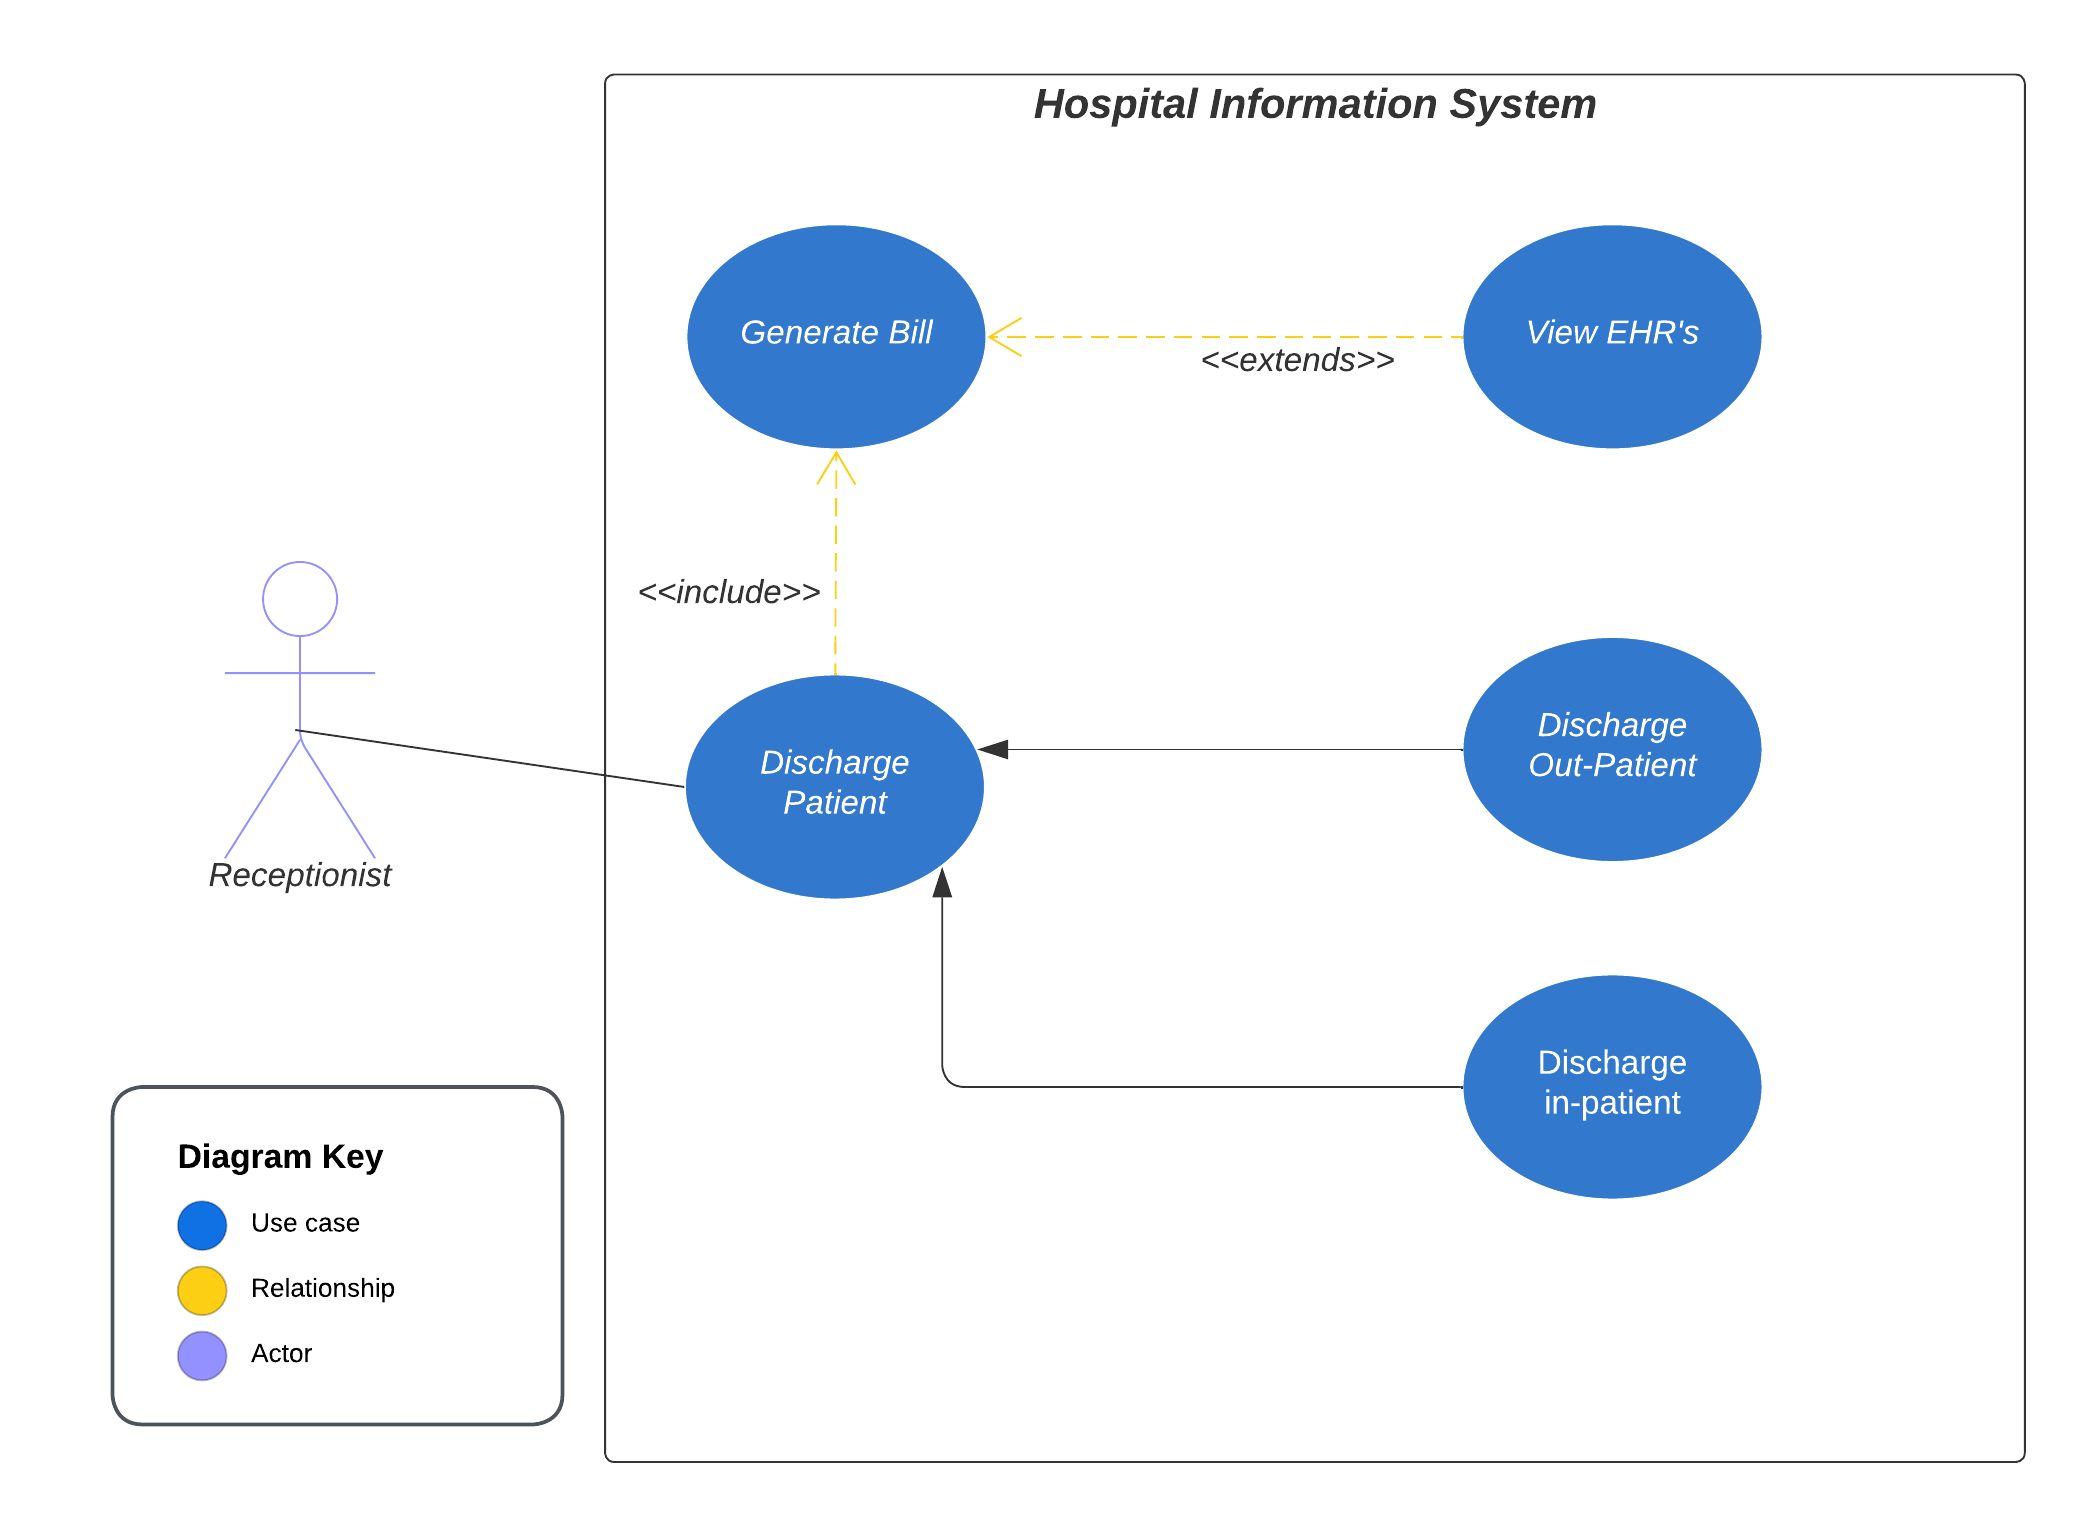
\includegraphics[width=12cm]{src/pic/Diagrams/Dischage_Patient_UCD.png}\end{center}
\caption{Visual Use Case Diagram of Discharge Patient Case}
\label{DPUCD}
\end{figure}


\subsection{Doctor Patient Interaction with EHR Use Case}

This use case diagram illustrates the interactions and functionalities of the Electronic Health Record (EHR) system within the hospital information system. It captures the use cases involving doctors and patients in accessing and managing medical information.

\textbf{Use Cases}
\begin{itemize}
    \item ViewMedicalHistory: This use case allows doctors and patients to view the medical history of the patient.
    \item AddDiagnosis: Doctors can use this use case to add a diagnosis to a patient's medical record.
    \item PrescribeMedication: Doctors can prescribe medication to patients using this use case.
    \item ScheduleAppointment: Patients can schedule an appointment using this use case.
    \item RequestMedication: Patients can request medication through this use case.
    \item ProvideMedicalHistory: Patients can provide their medical history using this use case.
\end{itemize}

\textbf{Actors}
\begin{itemize}
    \item Doctor: Represents the medical professional responsible for diagnosing and treating patients.
    \item Patient: Represents an individual seeking medical care from the hospital.
\end{itemize}

\textbf{Relationships}
\begin{itemize}
    \item The Doctor actor is associated with ViewMedicalHistory, AddDiagnosis, and PrescribeMedication use cases, indicating the functionalities available to doctors.
    \item The Patient actor is associated with ViewMedicalHistory, ScheduleAppointment, RequestMedication, and ProvideMedicalHistory use cases, representing the functionalities accessible to patients.
    \item ViewMedicalHistory extends ProvideMedicalHistory, indicating that the action of viewing the medical history is built upon the patient providing their medical history.
    \item PrescribeMedication includes RequestMedication, indicating that prescribing medication includes the request made by the patient.
\end{itemize}

\begin{figure}[!htb]
\lstset{language=MontiArc}
\lstinputlisting[
label=lst:docpat,
caption=Use Case Diagram in Moticore UCD for Doctor Patient Interaction with EHR Use Case] {src/listings/UCD/doctor_patient.ucd}
\end{figure}



\begin{figure}[!htb]
\begin{center}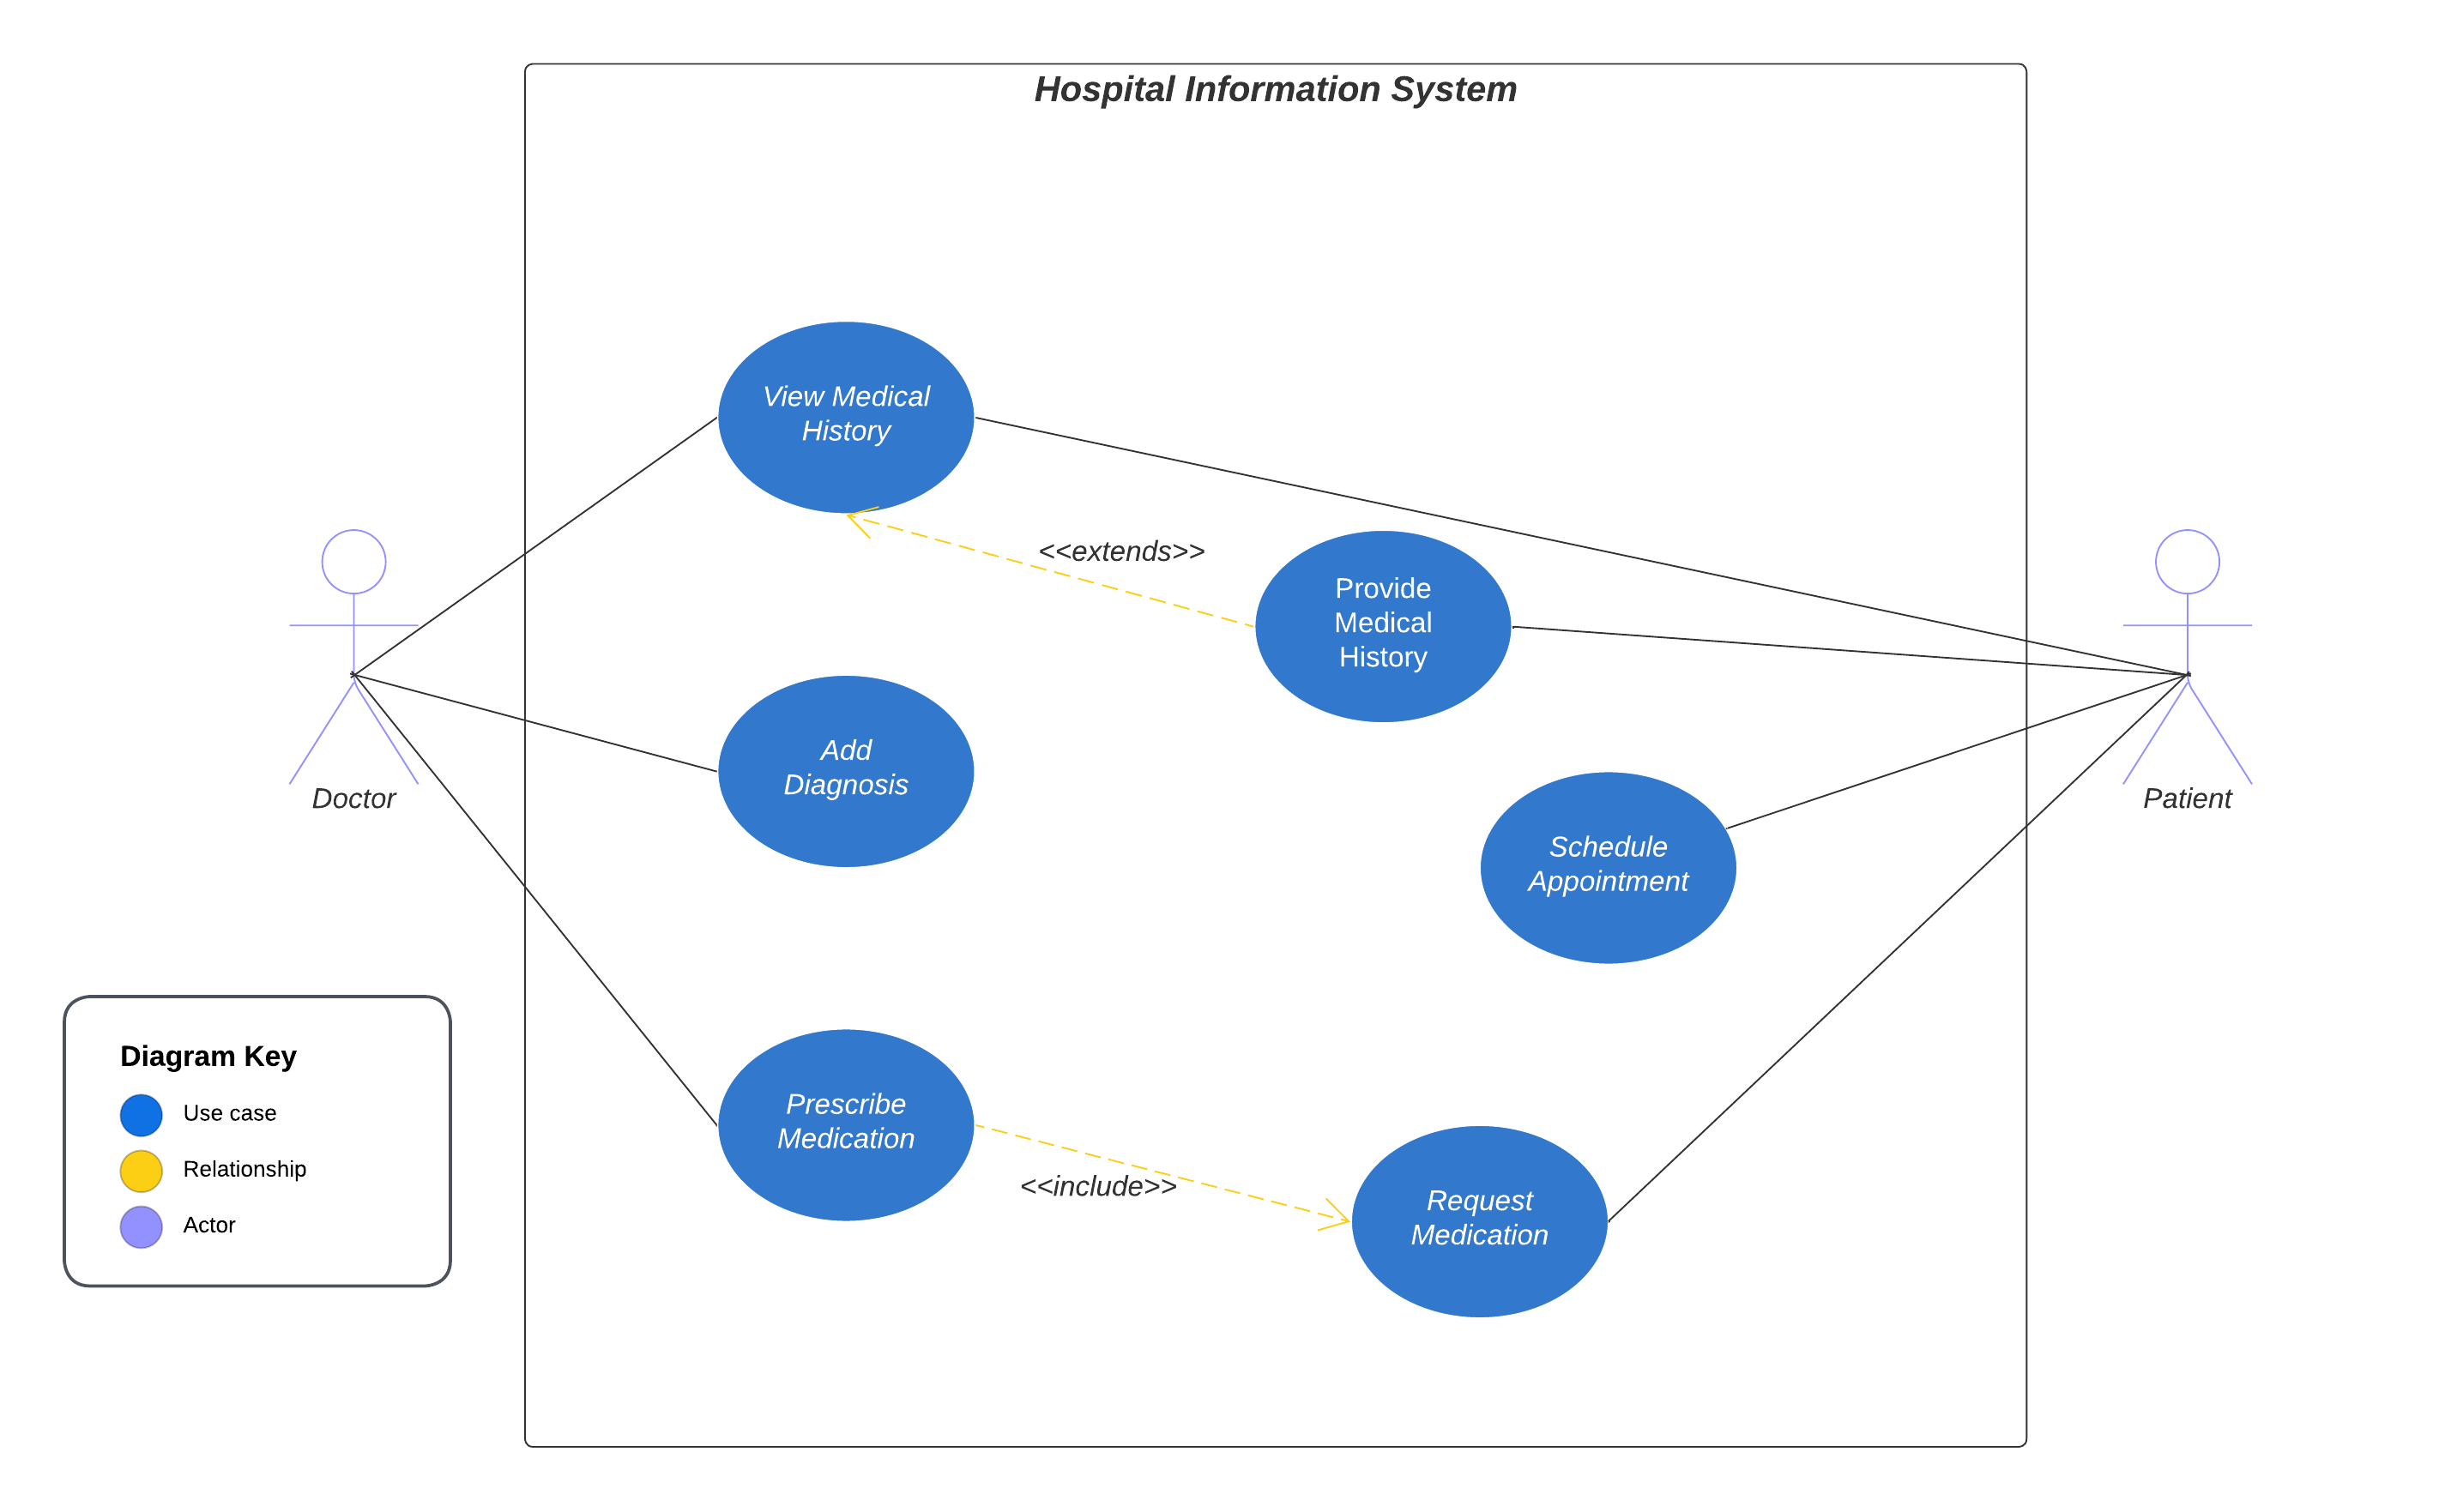
\includegraphics[width=12cm]{src/pic/Diagrams/EHR_Doctor_Patient_UCD.png}\end{center}
\caption{Visual Use Case Diagram of Doctor Patient Interaction with EHR Use Case}
\label{dopaUCD}
\end{figure}

\section{BPMN Diagram}

\begin{figure}[!htb]
\begin{center}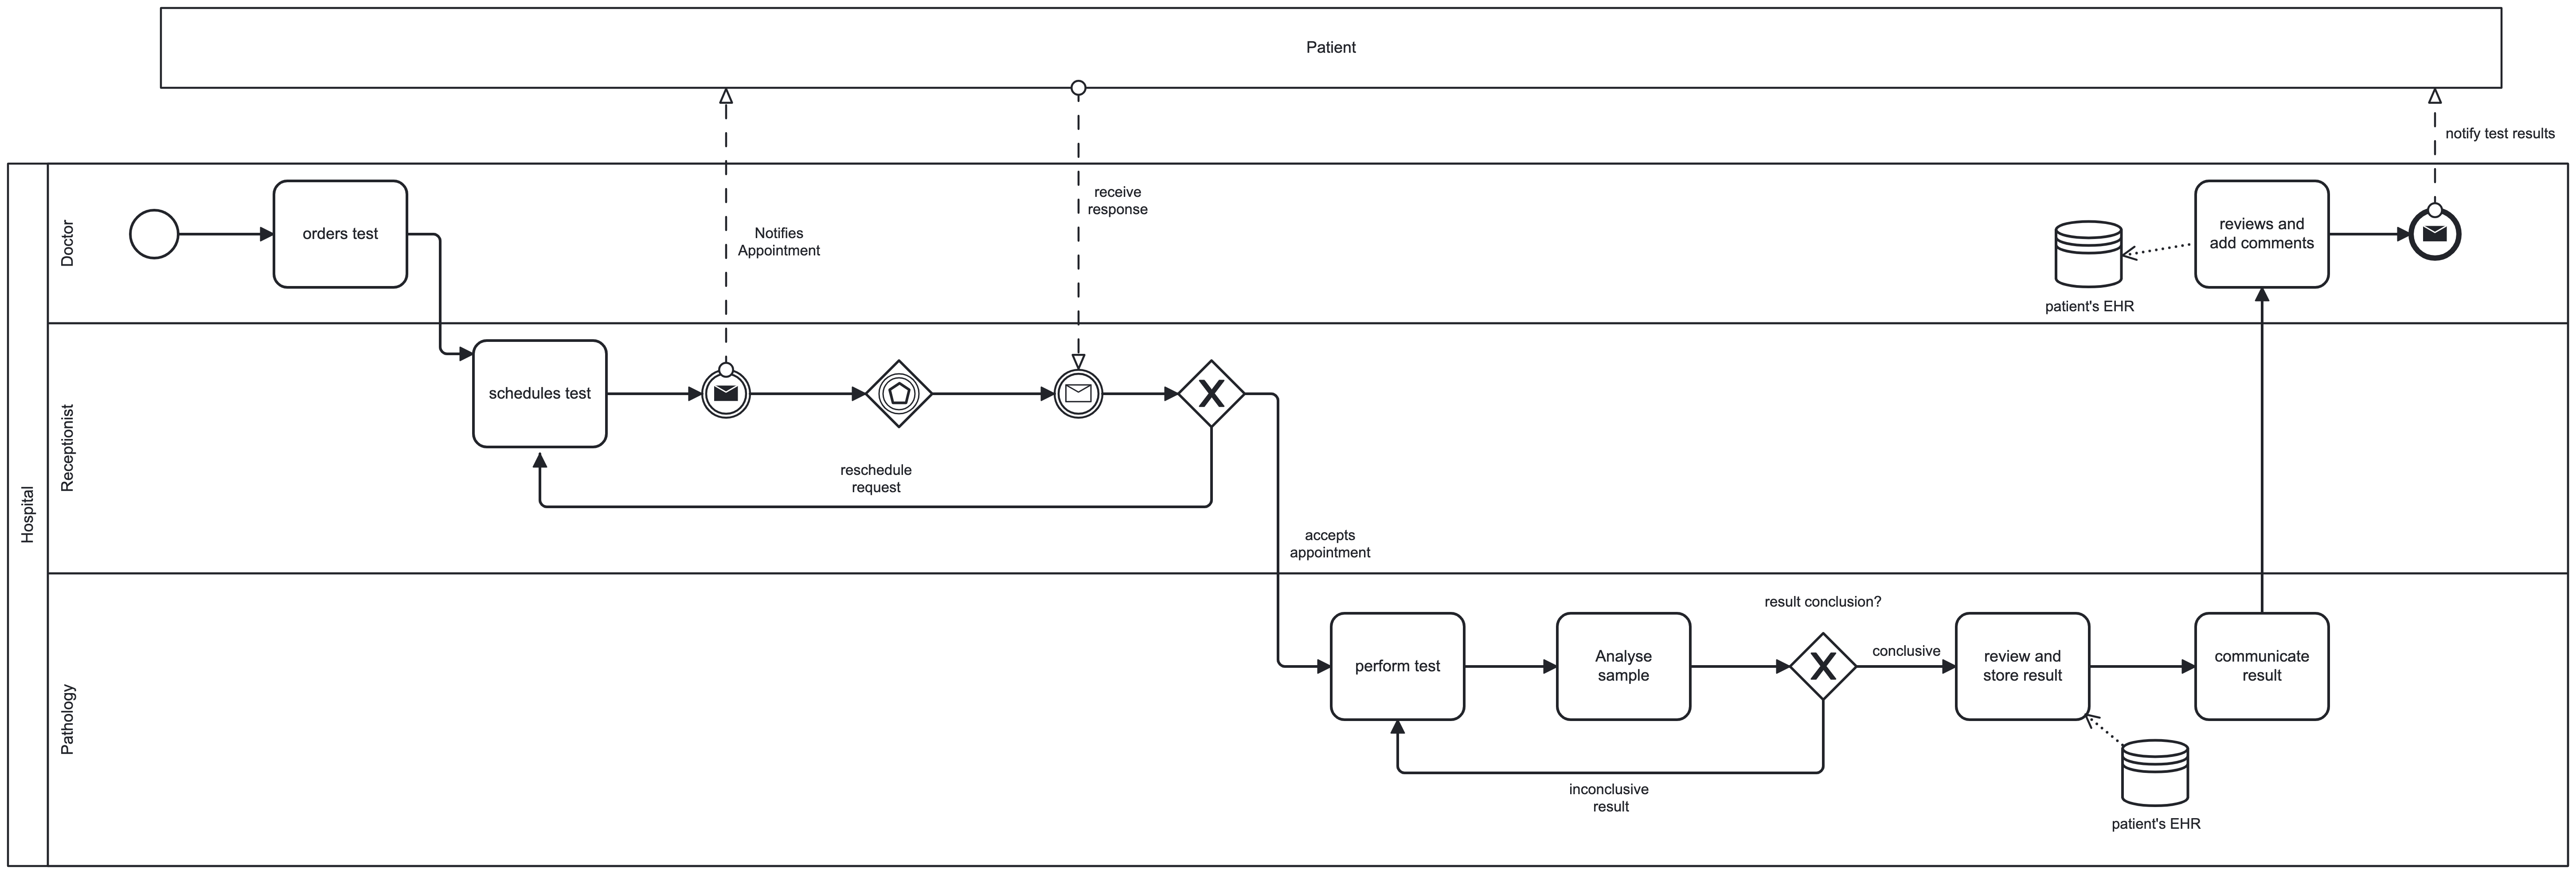
\includegraphics[width=20cm,angle=90]{src/listings/BPMN/lab_bmpn.png}\end{center}
\caption{BPMN Diagram showcasing the process of a doctor scheduling a test}
\label{bpmn}
\end{figure}

In the following BPMN model, the process of a doctor scheduling a test is explained:

\begin{enumerate}
\item The doctor in the hospital orders a test.
\item The receptionist receives the test order and schedules the test.
\item The receptionist notifies the patient about the scheduled appointment.
\item An event-based gateway is used to wait for the patient's response.
\item When the patient responds, it is checked if they want to reschedule the appointment or accept it.
\item If the patient wants to reschedule the appointment, the process loops back to the scheduling step.
\item If the appointment is accepted, the pathologist is assigned to perform the test.
\item The pathologist collects samples for the test and analyzes them.
\item If the test results are inconclusive, the test is performed again.
\item The pathologist repeats the test until the results are conclusive.
\item The conclusive test result is updated in the system and stored under the patient's electronic health record.
\item The test result is communicated to the doctor.
\item The doctor reviews the test result and updates the patient's health record in the health information system.
\item The doctor notifies the patient about the test result.
\end{enumerate}

\let\cleardoublepage\clearpage


\chapter{Related Works}
For related works, four papers are explored that either talked about Hospital Information Systems or Modelling various aspects of the Hospital Information System. 

The papers have approached the modeling of the E-health system using UML diagrams such as use case diagrams, activity diagrams, class diagrams, and component diagrams. The authors have identified several processes involved in clinical health services, including registration, polyclinic process, medicine, recipe, and doctor's schedule. They have integrated these processes to ensure that every patient who takes a medical check can register with only one registration and wait until called. 

The authors of the paper \textit{E-health as a Service Software of Medical System in UML
Modeling} have also identified some problems in the existing system, such as patients needing to be recorded in the insurance program provided by the government, causing trouble when searching for data. They have proposed a prototype modeling approach to construct the software, which is appropriate and straightforward. The prototype modeling approach allows the software to be delivered early, so the client can see the software and supervise the building of the software directly. 

They have also developed a component diagram that shows the application link among components built in the PHP language. They have created a class diagram that describes the system's structure, with classes having attributes, methods, and operations/methods. The classes in the system structure must be able to perform the functions in accordance with the system's needs. \cite{EHS}

The approach taken by the paper \textit{Health Information Systems} is to provide a comprehensive understanding of the management perspectives and inter-layer relationships of Hospital Information Systems (HIS). The authors propose three management perspectives: strategic, tactical, and operational, and describe their tasks and responsibilities. They also discuss the interlayer relationships between tasks and entity types, application components, and physical data processing components. The paper also introduces the PDCA (\textit{plan-do-check-act}) cycle and project management tools for organizing work in different phases. The result of the paper is a systematic approach to analyzing HIS, which can help hospital managers to make informed decisions about HIS implementation, operation, and maintenance.\cite{HIS}

The paper \textit{Modeling hospital information systems - Part 1: The revised three-layer graph-based meta model 3LGM2} presents a meta-model called 3LGM2 (\textit{Three Layer Graph Based Meta Model}) for modeling hospital information systems (HIS) using concepts on three layers: domain layer, logical tool layer, and physical tool layer. The approach is based on a case study that identified requirements for modeling HIS, and the meta-model was designed to meet those requirements. The paper also describes a software tool that supports the creation of 3LGM2 compliant models in a graphical way and can detect shortcomings at the logical or physical tool layers that make it impossible to satisfy the information needs at the domain layer.

The 3LGM2 meta-model is represented using the Unified Modeling Language and combines a functional meta-model with technical meta-models. It distinguishes between three different layers within an information system. It replaces the former 'procedure level' with the domain layer, which describes a hospital independently of its implementation by its enterprise functions. The logical tool layer focuses on application components, and the physical tool layer describes physical data processing components.

Compared to UML, the 3LGM2 approach has a lot of interlayer relationships and can be used as an ontology for describing HIS in natural language. However, the paper acknowledges some problems, such as the need for more process modeling and the considerable effort to model even a small information system from scratch. The paper concludes that reliable methods and tools can support hospital strategic information management. However, further evaluations on different sites are needed to show whether building and keeping up-to-date large models is possible.\cite{MHIS}

The paper \textit{UML-based ontology for describing hospital information system architectures} presents an ontology-based approach for describing hospital information systems architectures that allow the description of the essential information system components, their relationships, and their dependencies. The approach aims to answer relevant information management questions and provide criteria for the quality of a hospital information system. The ontology is presented using the Unified Modeling Language, and the examples are shown as intuitive graphical notations. 

The paper differs from other information systems planning and modeling approaches that place modeling aspects in the foreground, whereas interpretation and evaluation aspects are neglected. The presented ontology's selection of concepts for describing hospital information systems architectures and the relationships among these concepts is oriented towards information management questions that must be answered and information management tasks that must be supported in daily work. In comparison, the Unified Modeling Language is a general-purpose modeling language used in software engineering for visualizing, specifying, constructing, and documenting the artifacts of a software system. UML is not specific to hospital information systems but can be used to model any software system. The paper's approach is specific to hospital information systems and provides criteria for the quality of such systems.\cite{UHIS}

\let\cleardoublepage\clearpage
\chapter{Conclusion}
In conclusion, this research paper has presented a comprehensive analysis of modeling hospital information systems. By examining the various components of HIS, including electronic health records, and hospital billing and administrative systems, we have highlighted the critical role of modeling in designing and implementing effective healthcare information systems.

Through the utilization of modeling concepts such as Monticore and Business Process Model and Notation (BPMN), this paper has provided insights into the application of these techniques in capturing the structure, behavior, and interactions within hospital information systems. The use of Monticore has facilitated the creation of models such as class diagrams, use case diagrams, and sequence diagrams, while BPMN diagrams have enabled the representation of complex workflows and processes within the healthcare organization.

One of the notable strengths of the approach presented is the potential for reusability. The modeling techniques and concepts explored can serve as a foundation for future HIS projects, allowing stakeholders to build upon the existing knowledge and experience. The use of standardized notations and languages, such as UML and BPMN, enables interoperability and collaboration among different healthcare organizations and stakeholders.

Looking ahead, future work in this domain should address emerging challenges and leverage new technologies to further enhance the modeling and implementation of hospital information systems. For instance, advancements in artificial intelligence and machine learning can be harnessed to develop more intelligent clinical decision support systems. Additionally, the integration of Internet of Things (IoT) devices and wearable technologies into HIS modeling can enable real-time monitoring of patients and facilitate data-driven decision-making.

Furthermore, it is essential to continue exploring the ethical and legal considerations surrounding patient data privacy and security. With the increasing reliance on interconnected systems and the sharing of patient data, robust measures must be implemented to protect sensitive information and ensure compliance with relevant regulations.

By continuing to advance the modeling techniques and methodologies in hospital information systems, healthcare administrators, IT professionals, and researchers can contribute to the ongoing transformation of healthcare delivery, ultimately improving patient outcomes, streamlining workflows, and enhancing the overall quality of care.
% % Bild einbinden
% \begin{figure}[ht!]
% \begin{center}
\includegraphics[width=5cm]{src/pic/logo}\end{center}
% \caption{Das SE Logo}
% \label{Logo}
% \end{figure}

\let\cleardoublepage\clearpage


\bibliographystyle{alpha}
\addcontentsline{toc}{chapter}{Bibliography}
\bibliography{src/bib/Literatur}

% Begin Anhang
% \appendix
% \chapter{z.\,B. Programmdokumentation}

\cleardoublepage


\end{document}
